\documentclass{ieeeaccess}
\usepackage{cite}
\usepackage{amsmath,amssymb,amsfonts}
%\usepackage{algorithm}
\usepackage{algorithmic}
\usepackage[ruled, vlined, linesnumbered]{algorithm2e}
\usepackage{graphicx}
\usepackage{textcomp}

\usepackage{enumitem}

%Please add the following packages if necessary:
\usepackage{booktabs, multirow} % for borders and merged ranges
\usepackage{soul}% for underlines
\usepackage[table]{xcolor} % for cell colors
\usepackage{changepage,threeparttable} % for wide tables

\usepackage[commentmarkup=footnote,final]{changes} % Add changes for correction in text. USE THIS FOR FINAL VERSION
%\usepackage[commentmarkup=footnote]{changes} % Add changes for correction in text. USE THIS FOR REVIEW


\newcommand\Fig[1]{\textbf{Fig.}~\ref{#1}}
\newcommand\fig[1]{\textbf{Fig.}~\ref{#1}}
\newcommand\Tab[1]{\textbf{Tab.}~\ref{#1}}
\newcommand\tab[1]{\textbf{Tab.}~\ref{#1}}
\newcommand\Equ[1]{\textbf{Eq.}~(\ref{#1})}
\newcommand\equ[1]{\textbf{Eq.}~(\ref{#1})}
\newcommand\Sect[1]{\textbf{Sec.}~\ref{#1}}
\newcommand\sect[1]{\textbf{Sec.}~\ref{#1}}
\newcommand\Refs[1]{\textbf{Ref.}~\cite{#1}}
\newcommand\refs[1]{\textbf{Ref.}~\cite{#1}}
\newcommand\Algo[1]{\textbf{Algorithm}~\ref{#1}}
\newcommand\algo[1]{\textbf{Algorithm}~\ref{#1}}


\newcommand\todo[1]{\textbf{(TODO: {#1}})\\}

% To highlight "review"
%\newcommand\REVIEW[1]{\hl{#1}}
%To remove highlight
\newcommand\REVIEW[1]{{#1}}

\begin{document}
\history{Date of publication xxxx 00, 0000, date of current version xxxx 00, 0000.}
\doi{10.1109/ACCESS.2017.DOI}


\title {CNN Sensor Analytics with Hybrid-Float6 on Low-Power Resource-Constrained Embedded FPGAs.}

\author{
	\uppercase{Yarib Nevarez}\authorrefmark{1},
	\uppercase{Andreas Beering}\authorrefmark{1},
	\uppercase{Amir Najafi}\authorrefmark{1},
	\uppercase{Ardalan Najafi}\authorrefmark{1},
	\uppercase{Wanli Yu}\authorrefmark{1},
	\uppercase{Yizhi Chen}\authorrefmark{2},
	\uppercase{Karl-Ludwig Krieger}\authorrefmark{1},
	\uppercase{Alberto Garcia-Ortiz}\authorrefmark{1} \IEEEmembership{Member, IEEE},
}

\address[1]{Institute of Electrodynamics and Microelectronics, University of Bremen, Bremen 28359, Germany}

\address[2]{School of Electrical Engineering and Computer Science, KTH Royal Institute of Technology, 10044 Stockholm, Sweden}


\tfootnote{This work is funded by the Consejo Nacional de Ciencia y Tecnologia (CONACYT) and the Federal Ministry for Economic Affairs and Climate Action ZIM project IMOP (ZF4176708LP9).}

\markboth
{Author \headeretal: Preparation of Papers for IEEE TRANSACTIONS and JOURNALS}
{Author \headeretal: Preparation of Papers for IEEE TRANSACTIONS and JOURNALS}

\corresp{Corresponding author: Yarib Nevarez (e-mail: nevarez@item.uni-bremen.de).}

\begin{abstract}
The use of artificial intelligence (AI) in sensor analytics is entering a new era based on the use of ubiquitous embedded connected devices. This transformation requires the adoption of design techniques that reconcile accurate results with sustainable system architectures. As such, improving the efficiency of AI hardware engines as well as machine learning (ML) compatibility must be considered. In this paper, we present the Hybrid-Float6 (HF6) quantization and its dedicated hardware design. We propose an optimized multiply-accumulate (MAC) hardware by reducing the mantissa multiplication to a multiplexor-adder operation. We exploit the intrinsic error tolerance of neural networks to further reduce the hardware design with approximation. To preserve model accuracy, we present a quantization-aware training (QAT) method, which in some cases improves accuracy. We demonstrate this concept in 2D convolution layers. We present a lightweight tensor processor (TP) implementing a pipelined vector dot-product. For ML compatibility/portability, the 6-bit FP is wrapped in the standard FP format, which is automatically extracted by the proposed hardware. The hardware/software architecture is compatible with TensorFlow (TF) Lite. We evaluate the applicability of our approach with a CNN-regression model for anomaly localization in a structural health monitoring (SHM) application based on acoustic emission (AE). The embedded hardware/software framework is demonstrated on XC7Z007S as the smallest Zynq-7000 SoC. The proposed implementation achieves a peak power efficiency and acceleration of $5.7$ GFLOPS/s/W and $48.3\times$, respectively.
\end{abstract}

\begin{keywords}
Convolutional neural networks, structural health monitoring, hardware accelerator, TensorFlow Lite, embedded systems, FPGA, custom floating-point
\end{keywords}

\titlepgskip=-15pt

\maketitle
\chapter{Introduction}\label{chap.intro}
\minitoc
\section{Preamble}
\subsection{Industry 4.0}
Industry is the piece of an economy that produces material goods which are highly mechanized and automatized. Since the beginning of industrialization, technological leaps have led to paradigm shifts that are now called "industrial revolutions": from mechanization, electrification, and later, digitalization (the so-called 3rd industrial revolution). Based on the advanced digitalization within factories, the combination of Internet technologies and future-oriented technologies in the field of "smart" things (machines and products) seems to result in a new fundamental paradigm shift in industrial production. Emerging from this future expectation, the term "Industry 4.0" was established for an expected "4th industrial revolution" \cite{lasi2014industry}.


\subsection{Internet-of-Things in Industry}
% Context background
To build the emerging environment of Industry 4.0, disruptive technologies are required to handle autonomous communications between all industrial embedded computers throughout the factory and the Internet. Such technologies offer the potential to transform the industry along the entire production chain and stimulate productivity and overall economic growth \cite{espinoza2020estimating}. These technologies include cloud computing, big data, and specially a new generation of \gls{iot} devices fused with \gls{cps}, safety-security, augmented reality, hardware accelerators, and \gls{ai} in general \cite{alcacer2019scanning}.

\subsection{Artificial Intelligence in Internet-of-Things}
% Particular background
The continuous evolution of \gls{ai} algorithms and \gls{iot} devices has not only made \gls{ai} the major workload running on these embedded devices, but \gls{ai} has become the main approach for industrial solutions, especially in the rise of Industry 4.0 \cite{alcacer2019scanning}. In fact, there is a clear motivation to run \gls{ai}/\gls{ml} algorithms on \gls{iot} devices because of \cite{loh20201}: (1) feasibility of mission-critical real-time processing/inference; (2) privacy and security of data; (3) offline operation capability; and (4) robustness for stressed communication. Hence, the traditional term of \gls{iot} has also been redefined as AI of Things (AIoT) to emphasize the impact of \gls{ai}/\gls{ml} on this technology \cite{zhang2020empowering}.

\subsection{Error Tolerance in Machine Learning Algorithms}
An algorithm can be regarded as error-tolerant or error-resilient when it provides a result with the required accuracy while utilizing processing components with a certain degree of inaccuracy. There are several reasons why an algorithm/application is tolerant of errors as discussed in \cite{chippa2013analysis}. These include noisy or redundant data of the algorithm, approximate or probabilistic computations within the algorithm, and a range of acceptable outcomes. This is the case of \gls{ml} algorithms for \gls{ai} applications.

% Problem to solve
\section{Problem Statement}
The problem lies in the fact that state-of-the-art \gls{ai}/\gls{ml} algorithms, particularly \gls{ann}s, are highly compute and data intensive. This represents significant computational challenges across the spectrum of computing hardware, specially in the scope of embedded systems \cite{venkataramani2016efficient}. One of the most deployed applications is computer vision using \gls{cnn}s. Compared to the conventional image processing methods, the \gls{cnn} accuracy has improved significantly that by 2015, a human can no longer beat a computer in image classification \cite{loh20201}. The early development of \gls{cnn}s before 2016 mainly focused on accuracy improvement without considering computational costs. While accuracy of deep \gls{cnn} for image classification improved 24\% between 2012 and 2016, the demand on hardware resources increased more than $10\times$. Starting from 2017, significant attention was paid to improve hardware efficiency in terms of compute power, memory bandwidth, and power consumption, while maintaining accuracy at a similar level to human perception \cite{venkataramani2016efficient}.

% Consequences of the problem
Consequently, the recent breakthroughs in \gls{ai}/\gls{ml} applications have brought significant advancements in neural network processors \cite{jouppi2017datacenter}. These rapid evolution, however, came at the cost of an important demand for computational power. Hence, to bring the inference speed to an acceptable level, custom \gls{asic} with \gls{npu} are becoming ubiquitous in both embedded and general purpose computing. \gls{npu}s perform several tera operations per second in a confined area. Therefore, they become subject to elevated on-chip power densities that rapidly result in excessive on-chip temperatures during operation \cite{amrouch2020npu}.
These design efforts focused on power-hungry parallel computing techniques, yet unsustainable for resource-constrained devices.
As a result, radical changes to conventional computing approaches are required in order to sustain and improve performance while satisfying mandatory energy and temperature constraints \cite{gillani2020exploiting}.

In the state-of-the-art research, we find plenty of hardware architectures for \gls{cnn} accelerators implemented in \gls{fpga}. Most of the research implements fixed-point quantization, and very limited research focuses on \gls{fp}. Moreover, to the best of our knowledge, there is no research work exploring \gls{fp} inference for low-power embedded systems.

%%%%%%%%%%%%%%%%%%%%%%%%%%
\section{Research Objective}
The main objective for this doctoral research is investigating hardware design methodologies for low-power \gls{fp} neural network accelerators based on approximate computing in the scope of embedded systems.

%%%%%%%%%%%%%%
\section{Working Hypothesis}
% Alternatives and possible solutions for the problem
To overcome the problem, based on the error resilience of \gls{ml} algorithms, an evident solution is approximate computing. This computing paradigm has been used in a wide range of applications to increase the hardware computational efficiency \cite{han2013approximate}. For neural network applications, two main approximation strategies are used, namely network compression and classical approximate computing \cite{bouvier2019spiking}.

\subsection{Network Compression and Quantization}
Researchers focusing on embedded applications started lowering the precision of weights and activation maps to shrink the memory footprint of the large number of parameters representing \gls{ann}s, a method known as network quantization. In this manner, reduced bit precision causes a small accuracy loss \cite{courbariaux2015binaryconnect, han2015deep, hubara2017quantized, rastegari2016xnor}. In addition to quantization, network pruning reduces the model size by removing structural portions of the parameters and its associated computations \cite{lecun1989optimal,hassibi1992second}. This method has been identified as an effective technique to improve the efficiency of \gls{cnn} for applications with limited computational budget \cite{molchanov2016pruning,li2016pruning, liu2018rethinking}. These techniques leverage the intrinsic error-tolerance of neural networks, as well as their ability to recover from accuracy degradation while training.

\subsection{Approximate Computing}
%Geneal background
Approximate computing is an emerging design paradigm that is able to tradeoff computation quality (e.g., accuracy) and computational efficiency (e.g., in run-time, chip-area, and/or energy) by exploiting the error resilience properties of algorithms/applications \cite{gillani2020exploiting, zhang2015approxann}. Data redundancy of neural networks incorporate a certain degree of resilience against random external and internal perturbations, for instance, noisy inputs and random hardware errors. This property can be exploited in a cross-layer resilience approach \cite{carter2010design}: by leveraging error tolerance at algorithmic-level, it can be allowed a certain degree of inaccuracies at the computing-level. This approach consists of designing processing elements that approximate their computation by employing cleverly modified algorithmic logic units \cite{han2013approximate}.

Approximate computing techniques allow substantial enhancement in processing efficiency with moderated accuracy degradation. Some research papers have shown the feasibility of applying approximate computing to the inference stage of neural networks \cite{lotrivc2012applicability, han2013approximate, du2014leveraging, mrazek2016design, sarwar2016multiplier, zervakis2021approximate}. Such techniques usually demonstrated small inference accuracy degradation, but significant enhancement in computational performance, chip-area, and energy consumption. Hence, by taking advantage of the intrinsic error-tolerance of neural networks, approximate computing is positioned as a promising approach for inference on resource-limited devices. Nonetheless, the complex state-of-the-art of \gls{fp} \gls{cnn} inference has not been sufficiently explored with approximate computing techniques.

\section{Motivation}\label{chap1.motivation}
The use of \gls{ai}/\gls{ml} is entering a new era with ubiquitous embedded connected devices. This transformation requires design techniques that reconcile accurate results with cost-effective system architectures. However, state-of-the-art \gls{ai}/\gls{ml} algorithms represent high computational and energy costs. This compromises the sustainability of the progressive expansion towards massive ubiquitous \gls{ai} devices. Therefore, hardware efficiency is one of the major goals to innovate compute engines. This section presents the motivations to investigate design methodologies for low-power hardware acceleration for \gls{sbs} and \gls{cnn}s.

\subsection{Spike-by-Spike Neural Networks}

\gls{snn}s offer advantageous robustness and the potential to achieve a power efficiency closer to that of the human brain. \gls{snn}s operate reliably using stochastic elements that are inherently non-reliable mechanisms \cite{mcdonnell2011benefits}. This provides superior resistance against adversary attacks
\cite{ernst2007efficient, Dapello2020.06.16.154542}. Beside robustness, \gls{snn}s have further advantages like the possibility of a more efficient asynchronous parallelization and higher energy efficiency than conventional \gls{ann}s.

The Spike-by-Spike neural network is a remarkable model for its reduced complexity, which is on the less realistic side of the \gls{snn} scale of biological realism \cite{rotermund2019Backpropagation,ernst2007efficient}. Consequently, the hardware complexity of \gls{sbs} network implementations is greatly reduced \cite{rotermund2018massively}. In spite of this, \gls{sbs} still uses stochastic spikes as a means of transmitting information between populations of neurons and thus retains the advantageous robustness of \gls{snn}s. A significant research effort has been performed in \gls{snn} accelerators, see e.g. \cite{roy2019towards,bouvier2019spiking,
	young2019review,TrueNorth_Trans15,Spinnaker_Trans13,davies2018loihi}.

However, hardware accelerators that focus on \gls{sbs} have only been partially investigated so far \cite{rotermund2018massively}. Enhanced \gls{sbs} accelerators will have a double impact. From application point of view, they will contribute to the deployment of robust neural networks in small embedded systems \cite{nevarez2020accelerator}; from a scientific point of view, they will facilitate fundamental research for neuroscience \cite{ernst2007efficient,rotermund2019recurrentsbs, dayan2001theoretical}.

%%%%%%%%%%%%%%%%%%%%%%%%%%%%%%%%%%%%%%%%%%%%%%%%%%%%%%%%%%%%%%%%%%%%%%
\subsection{Convolutional Neural Networks}
\gls{cnn}s represent the essential building blocks in 2D pattern analytics. Sensor-based applications such as mechanical fault diagnosis \cite{li2019sensor,dong2018rolling}, structural health monitoring \cite{nagayama2007structural}, \gls{har} \cite{wang2019deep}, hazardous gas detection\cite{kim2017hazardous} have been powered by \gls{cnn} models in industry and academia. \gls{cnn} models provide advantages such as local dependency, scale invariance, and noise resilience in analytics\cite{du2014leveraging}. However, these models are computationally intensive and power-hungry. This is particularly challenging for low-power embedded applications in the field of \gls{iot}. As a result, numerous commercial \gls{asic} and \gls{fpga} accelerators have been proposed, targeting both \gls{hpc} for data-centers and embedded systems applications.

However, most accelerators have been implemented to target mid- to high-range \gls{fpga}s for computationally intensive \gls{cnn} models such as AlexNet, VGG-16, and ResNet-18. The main drawbacks of these implementations are power supply demands, physical dimensions, heat sink requirements, air cooling, and a resulting high price. In some cases, these implementations are not feasible for ubiquitous low-power/resource-constrained applications. Furthermore, reducing the compute hardware with aggressive quantization such as binary \cite{courbariaux2015binaryconnect}, ternary \cite{lin2015neural}, and mixed precision (2-bit activations and ternary weights) \cite{colangelo2018exploration} typically incur significant accuracy degradation for very low precisions, especially for complex problems\cite{faraone2019addnet}.

\section{Main Contribution}
This thesis contributes to hardware design methodologies for \gls{fp} neural network accelerators based on approximate computing in the scope of low-power embedded systems. The contributions for \gls{sbs} and \gls{cnn} hardware accelerators are listed below.

\subsection{Spike-by-Spike Neural Networks}
\begin{enumerate}
	\item We develop a hardware component for \gls{fp} vector dot-product approximation. This design increase the performance of computation by performing element-wise multiplication with a quality configurable design based on bit truncation and denormalized accumulation.
	\item We address a design exploration with the proposed dot-product approximation using synaptic weight vectors with custom \gls{fp} and logarithmic representation. We evaluate inference latency, accuracy degradation, resource utilization and power dissipation. Experimental results demonstrate $20.5\times$ latency enhancement versus embedded CPU (ARM Cortex-A9 at $666$MHz), and less than $0.5\%$ of accuracy degradation on a handwritten digit recognition task (MNIST).
	\item We propose a noise tolerance plot as quality monitor, which serves as an intuitive visual model to provide insights into the accuracy degradation of \gls{sbs} networks under approximate processing effects.
	\item Our proposed design for \gls{fp} dot-product approximation is adaptable as a building block for other error resilient applications (e.g., image/video processing).
\end{enumerate}


\subsection{Convolutional Neural Networks}
\begin{enumerate}
	\item
	
	We present the \gls{hf6} quantization and its dedicated hardware design. We propose an optimized hardware \gls{mac} by reducing the mantissa multiplication to a multiplexer-adder operation. We exploit the intrinsic error tolerance of \gls{ann} to further reduce the hardware design with approximation. To preserve model accuracy, we present a quantization-aware training method, which in some cases improves accuracy.
	
	\item We develop a custom hardware/software co-design framework for sensor analytics applications on low-power embedded \gls{fpga}s. This architecture integrates TensorFlow Lite.
	\item We present a customizable tensor processor as a dedicated hardware for \gls{hf6}. This design computes \emph{Conv2D} tensor operations employing a pipelined vector dot-product with parametrized on-chip memory utilization.
	\item We demonstrate the potential of our approach with a \gls{cnn}-regression model for anomaly localization in structural health monitoring based on acoustic emissions. We address a hardware design exploration evaluating accuracy, compute performance, hardware resource utilization, and energy consumption.
\end{enumerate}

\section{Publications}
The outcome of the research of this dissertation, including the collaborative works with our research partners is a list of publications including \cite{nevarez2020accelerator, nevarez2021accelerating, yu2020taac}. In the following, a complete list of the related publications are itemized.

\begin{enumerate}
	
	\subsubsection*{Journal Articles}
	
	\item \textbf{Yarib Nevarez}, David Rotermund, Klaus R Pawelzik, and Alberto Garcia-Ortiz, "Accelerating Spike-by-Spike Neural Networks on FPGA With Hybrid Custom Floating-Point and Logarithmic Dot-Product Approximation," 
	\newblock IEEE Access, vol. 9, pp. 80603--80620, May 2021, doi: 10.1109/ACCESS.2021.3085216.  
	
	\item \textbf{Yarib Nevarez}, David Rotermund, Klaus R Pawelzik, and Alberto Garcia-Ortiz, "CNN Sensor Analytics with Hybrid-Float6
	on Low-Power Resource-Constrained
	Embedded FPGAs.," 
	\newblock IEEE Access, vol. 9, pp. 80603--80620, May 2021, doi: 10.1109/ACCESS.2021.3085216.

	
	\subsubsection*{Conference Proceedings}
	
	\item \textbf{Yarib Nevarez}, Alberto Garcia-Ortiz, David Rotermund, and Klaus R Pawelzik, "Accelerator framework of spike-by-spike neural networks for inference and incremental learning in embedded systems,"
	\newblock 2020 9th International Conference on Modern Circuits and Systems Technologies (MOCAST), Bremen, 2020, pp. 1--5, doi: 10.1109/MOCAST49295.2020.9200288.
	
	\item Wanli Yu, Ardalan Najafi, \textbf{Yarib Nevarez}, Yanqiu Huang and Alberto Garcia-Ortiz, "TAAC: Task Allocation Meets Approximate Computing for Internet of Things," 
	\newblock 2020 IEEE International Symposium on Circuits and Systems (ISCAS), Sevilla, 2020, pp. 1-5, doi: 10.1109/ISCAS45731.2020.9180895.
	
	\item Amir Najafi, Ardalan Najafi, \textbf{Yarib Nevarez} and Alberto Garcia-Ortiz, "Learning-Based On-Chip Parallel Interconnect Delay Estimation," 
	\newblock 2022 11th International Conference on Modern Circuits and Systems Technologies (MOCAST), Bremen, 2022, pp. 1--5, doi: 10.1109/MOCAST49295.2020.9200288.
	
\end{enumerate}

\section{Dissertation Outline}

This dissertation is organized in three main parts: an introduction, where
the state of the art and related background are stated; a central core, where the proposed design methodologies and validation are presented; and a final part with the conclusion. More precisely:

\begin{enumerate}[I]
	\item \textbf{Introduction}: Chapter~\ref{chap.background} introduces the background related to \gls{sbs}, \gls{cnn}, and \gls{fp} number representation.
	\item \textbf{Core}: the proposed hardware design methodologies for \gls{sbs} and \gls{cnn} accelerators are presented in Chapter~\ref{chap.sbs} and Chapter~\ref{chap.cnn}, respectively.
	\item \textbf{Conclusions}: the final conclusions are presented in Chapter~\ref{chap.conclusion}.
\end{enumerate}
\section{Related Work}
\label{sec:related_work}
%%%%%%%%%%%%%%%%%%%%%%%%%%%%%%%%%%%%%%%%%%%%%%%%%%%%%%
For efficient neural network computation, two main optimization strategies are used, namely network compression and classical approximate computing~\cite{bouvier2019spiking}.

\subsection{Network Compression}
Researchers focusing on embedded applications started lowering the precision of weights and activation maps to shrink the memory footprint of the large number of parameters representing \glspl{ann}, a method known as network compression or quantization. This practice takes advantage of the intrinsic error-tolerance of neural networks, as well as their ability to compensate for approximation while training. In this way, reduced bit precision causes a small accuracy loss~\cite{courbariaux2015binaryconnect, han2015deep, hubara2017quantized, rastegari2016xnor}.

In hardware development, \gls{wq} has shown up to $2\times$ improvement in energy consumption with an accuracy degradation of less than $1\%$ \cite{moons20160, whatmough201714}. Some advanced quantization methods yield to \glspl{bnn} allowing the use of \glspl{xnor} instead of the conventional costly \glspl{mac}~\cite{rastegari2016xnor}. In~\cite{sun2018xnor}, Sun et al. report an accuracy of $98.43\%$ on handwritten digit classification (MNIST) with a simple \gls{bnn}. Hence, quantization is a powerful tool for improving the energy efficiency and memory requirements of \gls{ann} accelerators, with limited accuracy degradation.

In addition to quantization, network pruning reduces the model size by removing structural portions of the parameters and its associated computations~\cite{lecun1989optimal,hassibi1992second}. This method has been identified as an effective technique to improve the efficiency of \gls{dnn} for applications with limited computational budget~\cite{molchanov2016pruning,li2016pruning, liu2018rethinking}.

These methods can be used for \glspl{snn} as well. In~\cite{rathi2018stdp}, Rathi et al. report up to $3.1\times$ improvement in energy consumption with an accuracy loss of around $3\%$. Weight quantization allows the designer to realize a trade-off between the accuracy of the \gls{snn} application and efficiency of resources. Approximate computing can also be applied at the neuron level, where irrelevant units are deactivated to reduce the computation cost of the \glspl{snn}~\cite{sen2017approximate}. This computation skipping can be applied randomly on synapses, training \glspl{ann} with stochastic synapses improves generalization, resulting in a better accuracy~\cite{srivastava2014dropout, wan2013regularization}. Such methods are compatible with \glspl{snn} and have been tested both during training~\cite{neftci2016stochastic, srinivasan2016magnetic} and operation \cite{buesing2011neural}, and even to define the connectivity between layers \cite{bellec2017deep, chen20184096}. Implementations of spiking neuromorphic systems in FPGA~\cite{sheik2016synaptic} and hardware~\cite{jerry2017ultra} demonstrated that synaptic stochasticity allows to increase the final accuracy of the networks while reducing memory footprint.

Quantization is therefore a powerful technique to improve energy efficiency and memory requirements of \gls{ann} and \gls{snn} accelerators, with small accuracy degradation. However, this approach requires quantization-aware training methods that, in some cases, are problematic or even inaccessible, particularly in emerging deep \gls{snn} algorithms~\cite{zhang2018survey}.

\subsection{Classical Approximate Computing}
Approximate computing has been used in a wide range of applications to increase the computational efficiency in hardware\cite{han2013approximate}. This approach consists of designing processing elements that approximate their computation by employing modified algorithmic logic units \cite{han2013approximate}. In~\cite{kim2013energy}, Kim et al. have shown \glspl{snn} using carry skip adders achieving $2.4\times$ latency enhancement and $43\%$ more energy efficiency, with an accuracy degradation of 0.97\% on a handwritten digit classification task (MNIST). Therefore, approximate computing provides important enhancement in energy efficiency and processing speed.

However, as the complexity of the dataset increases, as well as the depth of the network topology, such as ResNet~\cite{he2016deep} on ImageNet~\cite{russakovsky2015imagenet}, the accuracy degradation becomes more important and may not be negligible anymore \cite{rastegari2016xnor}, especially for critical applications such as autonomous driving. Therefore, it is not certain that network compression techniques and approximate computing are suitable for all applications.

\subsection{Spike-by-Spike Neural Networks Accelerators}
Recently, Rotermund et al. demonstrated the feasibility of a neuromorphic \gls{sbs} \gls{ip_sbs} on a Xilinx Virtex 6 \gls{fpga}~\cite{rotermund2018massively}. It provides a massively parallel architecture, optimized to reduce memory access and suitable for \gls{asic} implementations. Nonetheless, this design is considerably resource-demanding if implemented as a full \gls{sbs} network in today's embedded technology.
%%%%%%%%%%%%%%%%%%%%%%%%%%%%%%%%%%%%%%%%%%%%%%%%%%%%%%
\chapter{Background}\label{chap.background}
\minitoc

\section{Spike-by-Spike Neural Networks} 

\label{sec:sbs}

Technically, \gls{sbs} is a spiking neural network approach based on a
generative probabilistic model. It iteratively finds an estimate of
its input probability distribution $p(s)$ (i.e. the probability of
input node $s$ to stochastically send a spike) by its latent variables
via $r(s) = \sum_i h(i) W(s|i)$. 
where $\vec{h}$ is an inference
population composed of a group of neurons that compete with each
other. An \gls{ip_sbs} sees only the spikes $s_t$ (i.e. the
index identifying the input neuron $s$ which generated that spike at
time $t$) produced by its input neurons, not the underlying input
probability distribution $p(s)$ itself. By counting the spikes
arriving at a group of \gls{sbs} neurons, $p(s)$ is estimated by
$\hat{p}(s) = 1/T \sum_t \delta_{s,s^t}$ after $T$ spikes have been
observed in total. The goal is to generate an internal representation
$r(s)$ from the string of incoming spikes $s_t$ such that the negative
logarithm of the likelihood
$L = C - \sum_\mu \sum_s \hat{p}_\mu(s) log\left( r_\mu(s) \right)$ is
minimized. $C$ is a constant which is independent of the internal
representation $r_\mu(s)$ and $\mu$ denotes one input pattern from an
ensemble of input patterns. Applying a multiplicative gradient descent
method on $L$, an algorithm for iteratively updating $h_\mu(i)$ with
every observed input spike $s_t$ could be derived
\cite{ernst2007efficient}
\begin{eqnarray} \label{eq:sbs_update}
h_\mu^{new}(i) = \frac{1}{1+\epsilon} \left(h_\mu(i) + \epsilon \frac{h_\mu(i) W(s_t|i) }{\sum_j h_\mu(j) W(s_t|j)} \right) 
\end{eqnarray}
where $\epsilon$ is a parameter that also controls the strength of sparseness of the distribution of latent variables $h_\mu(i)$. Furthermore, $L$ can also be used to derive online and batch learning rules for optimizing the weights $W(s|i)$. The interested reader is referred to \cite{ernst2007efficient} for a more detailed exposition.

From a practical point of view, \gls{sbs} provides a mechanism to obtain a sparse representation of input patterns. Given a set of
	training samples $\{x_\eta\}$, it learns weights ($W$), that allow
	to express the input patterns as a linear sparse non-negative combination
	of features.  During inference, it provides a mechanism for expressing
	each test input $x_\mu$ as $x_\mu \approx W\, h_\mu$ where all
	entries are non-negative.
	
	The inference procedure consists in generating indices $s_t$
	distributed according to a categorical distribution of the input pattern
	$s_t \sim \mathrm{Categorical}(x_{\mu}(0), x_{\mu}(1), ..,
	x_{\mu}(N-1))$. Starting with a random $h$ and executing
	iteratively \Equ{eq:sbs_update} the \gls{sbs} algorithms finds
	$h_{\mu}$. The fundamental concept of \gls{sbs} can be extended from vector to matrix
	inputs. In this case, the linear operation $W\, h_\mu$ can be replaced by a
	convolution to obtain a convolutional \gls{sbs} layer. A detailed description of the \gls{sbs} algorithm is presented in the Appendix~\ref{chap.append}

\subsection{Basic Network Overview}

\gls{sbs} network models can be constructed in sequential layered structures \cite{rotermund2019Backpropagation}. Each layer consists of many \gls{ip_sbs}s (represented by $\vec{h}$), while the communication between them is organized by a low bandwidth signal -- the spikes.

The \gls{sbs} layer update is summarized in Algorithm~\ref{alg:sbs}. This is an iterative algorithm, where we denote the number of spikes ($N_{Spk}$) as the number of iterations. As a generative model, each iteration updates the internal representation ($H$) based on the input spikes ($S^{in}_t$). A basic \gls{sbs} network architecture for handwritten digit classification (MNIST) is shown in \fig{fig:sbs_network} and \Tab{tab:sbs_network}. Each \gls{ip_sbs} is an independent computational entity, this allows to design specialized hardware architectures that can be massively parallelized (see \fig{fig:SbS_layer}).


\begin{algorithm}[b!]
	\caption{SbS layer update.}\label{alg:sbs}
	
	\begin{algorithmic}[1]
		\FOR {$t \leftarrow 0$ \textbf{to} $N_{Spk}-1$}
		\FOR {$x \leftarrow 0, y \leftarrow 0$ \textbf{to} $N_X-1, N_Y - 1$}
		\STATE $S^{out}_t(x, y) \sim Categorical( H^{}(x, y, :) ) $
		\FOR {$\Delta_X \leftarrow 0, \Delta_Y \leftarrow 0$ \textbf{to} $K_X - 1,K_Y - 1$}
		\STATE $spk \leftarrow S^{in}_t(x + \Delta_X , y + \Delta_Y)$
		\FOR {$i \leftarrow 0$ \textbf{to} $N_H-1$}
		\STATE $\Delta h(i)
		\leftarrow H^{}(x, y,  i) \cdot W^{}(\Delta_X, \Delta_Y, spk, i)$
		\STATE $r \leftarrow r + \Delta h(i)$
		\ENDFOR
		
		\FOR {$i \leftarrow 0$ \textbf{to} $N_H-1$}
		\STATE $H^{new}(x, y, i) \leftarrow \frac{1}{1+\epsilon} \left( H^{}(x, y, i) + \frac{\epsilon}{r} \Delta h(i) \right) $              
		\ENDFOR
		\ENDFOR
		\ENDFOR
		\ENDFOR
	\end{algorithmic} 
\end{algorithm}

\begin{figure*}[b!]
	\centering
	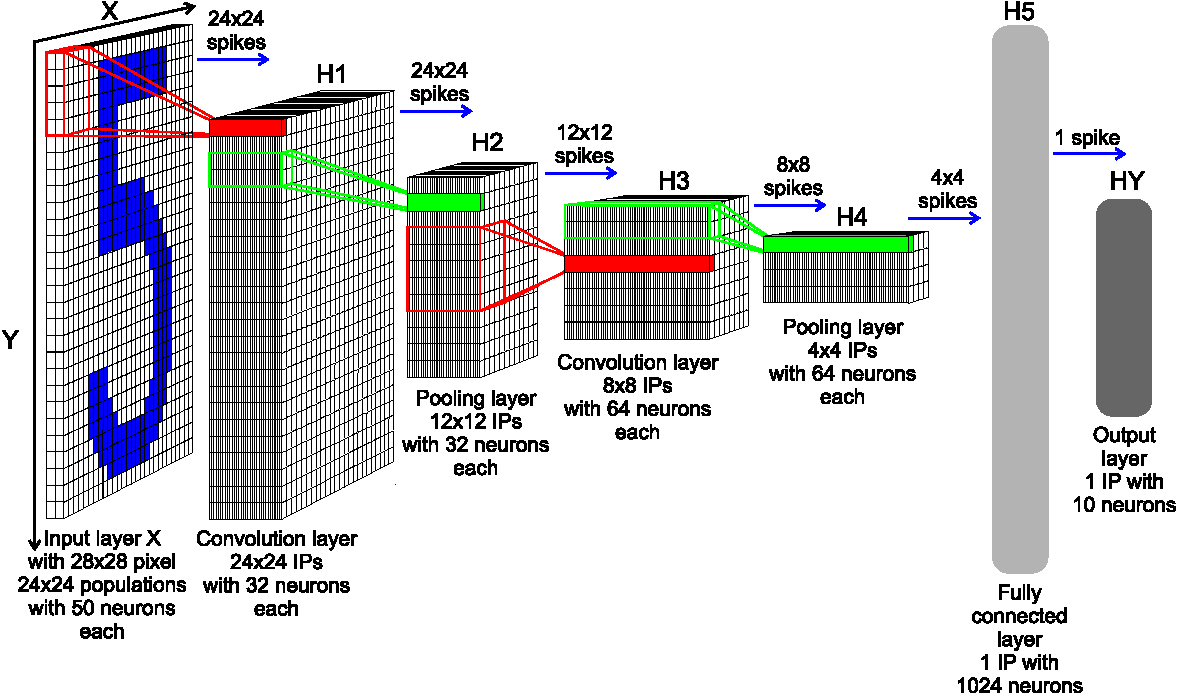
\includegraphics[width=0.5\columnwidth]{./chapters/sbs_accelerator/figures/sbs_network.pdf}
	\caption{\gls{sbs} network architecture for handwritten digit classification task.}
	\label{fig:sbs_network}
\end{figure*}


\begin{table}[t!]\centering
	\caption{\gls{sbs} network architecture for handwritten digit classification task.}
	\label{tab:sbs_network}
	\scriptsize
	\begin{tabular}{lrrrrrrr}\toprule
		&\multicolumn{3}{c}{\textbf{Layer size}} & &\multicolumn{2}{c}{\textbf{Kernel size}} \\\cmidrule{2-4}\cmidrule{6-7}
		\textbf{Layer} ($H^l$) &$N_X$ &$N_Y$ &$N_H$ & &$K_X$ &$K_Y$ \\\midrule
		Input ($HX$) &28 &28 &2 & &- &- \\
		Convolution ($H1$) &24 &24 &32 & &5 &5 \\
		Pooling ($H2$) &12 &12 &32 & &2 &2 \\
		Convolution ($H3$) &8 &8 &64 & &5 &5 \\
		Pooling ($H4$) &4 &4 &64 & &2 &2 \\
		Fully connected ($H5$) &1 &1 &1024 & &4 &4 \\
		Output ($HY$) &1 &1 &10 & &1 &1 \\
		\bottomrule
	\end{tabular}
\end{table}

\subsection{Computational Cost}

The number of \gls{mac} operations required for inference of an \gls{sbs} layer is defined by $NOPS_{MAC}=N_{Spk} N_X N_Y K_X K_Y (3 N_H + 2)$, where $N_{Spk}$ is the number of spikes (iterations), $N_X N_Y$ is the size of the layer, $K_X K_Y$ is the size of the kernel for convolution/pooling, and $N_H$ is the length of $\vec{h}$. The computational cost of \gls{sbs} network models is higher compared to equivalent \gls{cnn} models and lower compared to regular \gls{snn} models (e.g., \gls{lif}) \mbox{\cite{izhikevich2004model}}.


\begin{figure*}[b!]
	\centering
	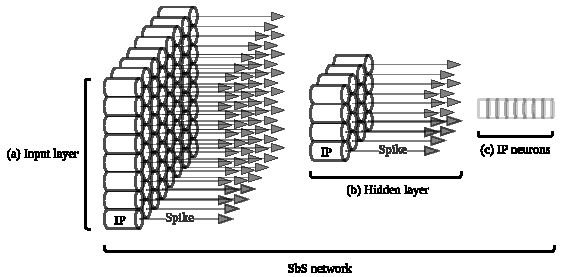
\includegraphics[width=0.5\columnwidth]{./chapters/sbs_accelerator/figures/SbS_layer.pdf}
	\caption{\gls{sbs} \gls{ip_sbs}s as independent computational entities, (a) illustrates an input layer with a massive amount of \glspl{ip_sbs} operating as independent computational entities, (b) shows a hidden layer with an arbitrary amount of \gls{ip_sbs}s as independent computational entities, (c) exhibits a set of neurons grouped in an \gls{ip_sbs}.}
	\label{fig:SbS_layer}
\end{figure*}


\subsection{Error Tolerance}

To illustrate the error tolerance/resilience of \gls{sbs} networks, we present a classification performance under positive additive uniformly distributed noise as external disturbance. \fig{fig:robustnes_sbs} presents a comparison of the classification performance of an \gls{sbs} network and a standard \gls{cnn}, with the same amount of
neurons per layer as well as the same layer structure. We trained both neural networks for handwritten digit classification on MNIST dataset \cite{lecun1998mnist} (see \cite{rotermund2019Backpropagation} for details). The figure shows the correctness for the MNIST test set with its \num[group-separator={,}]{10000} patterns in dependency of the noise level for positive additive
uniformly distributed noise. The blue curve shows the performance for
the \gls{cnn}, while the red curve shows the performance for
the \gls{sbs} network with \num[group-separator={,}]{1200} spikes (iterations). Beginning
with a noise level of 0.1, the respective performances are different
with a p - level of at least $10^{-6}$ (tested with the Fisher exact
test). Increasing the number of spikes per \gls{sbs} population to \num[group-separator={,}]{6000}
(performance values shown as black stars), shows that more spikes can
improve the performance under noise even more.

\begin{figure*}[b!]
	\centering
	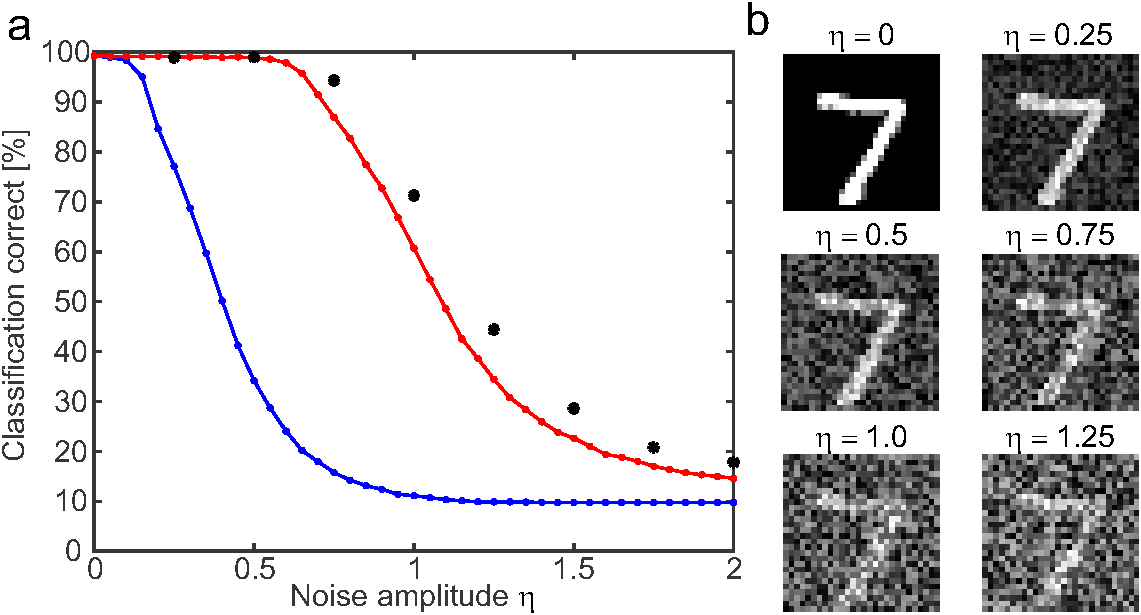
\includegraphics[width=0.5\columnwidth]{./chapters/sbs_accelerator/figures/sbs_robustnes.pdf}
	\caption{(a) Performance classification of \gls{sbs} NN versus equivalent \gls{cnn}, and (b) example of the first pattern in the MNIST test data set with different amounts of positive additive uniformly distributed noise.}
	\label{fig:robustnes_sbs}
\end{figure*}

%%%%%%%%%%%%%%%%%%%%%%%%%%%%%%%%%%%%%%%%%%%%%%%%%%%%%%%%%%%%%%%%%%%%%%%%%%%%%%%%%%%%%%
\section{Conv2D Tensor Operation}
A convolutional layer aims to learn feature representations from an input layer. The convolution layer is made of convolution kernels that are used to compute feature maps. Each unit of a feature map is connected to a region of neighboring units on the input maps (from previous layer). Such a neighborhood of the previous layer is known as the receptive field of the unit. A new feature map can be obtained by first convolving the input maps with a learned kernel and then applying a nonlinear elementwise activation function to the convolved results. All spatial locations on the input maps share a kernel to generate a feature map. All feature maps are obtained by convolving several different kernels~\cite{gu2018recent}.


The 2D convolution process is performed by the \emph{Conv2D} tensor operation, described in \Equ{eq:conv2D}, where $h$ is the input tensor containing the feature maps, $W$ is the convolution kernels (known as filters), and $b$ is the bias vector for the output feature maps~\cite{goodfellow2016deep}. $K\times L\times M$ is the receptive field size, $K\times L$ is the convolution kernel, and $M$ is the number of input channels/feature maps. We denote \emph{Conv} as \emph{Conv2D} operator.
\begin{eqnarray} \label{eq:conv2D}
Conv\left(W,h\right)_{i,j,o}=\sum_{k,l,m}^{K,L,M} h_{(i+k,j+l,m)} W_{(o,k,l,m)}+b_{o}
\end{eqnarray}

\section{Floating-point Number Representation}
The representation of every numerical value, in any number system, is made of an integer and a fractional part. The border that delimits them is called the radix point. The fixed-point format for representing numeric values derives its name from the fact that in this format, the base point is fixed at a certain position. For integer numbers, this position is at the right of the least significant digit.

In scientific computation, it is often necessary to represent very large and very small values. This is difficult to achieve using the fixed-point format because the bit size/width required to maintain both the desired precision and the desired range are very large. In such situations, \gls{fp} formats are used to represent real numbers. Each \gls{fp} number can be divided into three fields: sign $S$, exponent $E$, and mantissa $M$. Using the binary number system, it is possible to represent any \gls{fp} number as:

\begin{eqnarray} \label{eq:float}
(-1)^{S} \times 1.M \times 2^{E-B}
\end{eqnarray}

In \gls{fp} representations the exponent is biased. This bias depends on the bit size of the exponent field in the particular format. This exponent bias is defined by \Equ{eq:float_bias}, where $E_{size}$ is the exponent bit size.

\begin{eqnarray} \label{eq:float_bias}
B=2^{E_{size}-1}-1
\end{eqnarray}

There is a natural trade-off between small bit size requiring fewer hardware resources and larger bit size providing higher precision. Within a given total bit size, it is possible to assign various combinations of sizes to the exponent and mantissa fields, with wider exponents resulting in a higher range and wider mantissa resulting in better precision.

The most widely used format for \gls{fp} arithmetic is the IEEE 754 standard \cite{zuras2008ieee}. The IEEE single-precision format (32-bit) is expressed by \Equ{eq:float} with $B$ = 127, 8 bits for the exponent and 23 bits for the mantissa, see \Fig{fig:floating}(a). In \gls{fp} formats, the numbers are normalized, the leading one is an implicit bit, and only the fractional part is explicitly stored in the mantissa field.

\begin{figure*}[b!]
	\centering
	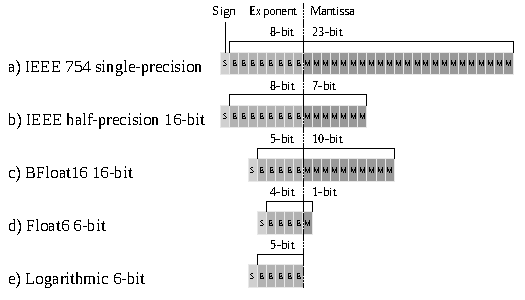
\includegraphics[width=0.5\columnwidth]{./chapters/cnn_accelerator/figures/power_breakdown/floating_point.pdf}
	\caption{Floating-point number representation.}
	\label{fig:floating}
\end{figure*}

Reduced bit size than those specified in the IEEE 754 standard are often sufficient to provide the desired precision. Reduced designs require fewer hardware resources enabling low-power implementations. In custom hardware designs, it is possible to customize the \gls{fp} format implemented. In later sections, we use the term E$a$M$b$ to denote \gls{fp} formats, where $a$ and $b$ are the exponent and mantissa bit size, respectively. For example, E4M1 means 4-bit exponent and 1-bit mantissa, see \Fig{fig:floating}(d).

There are three special definitions in IEEE 754 standard. The first is subnormal numbers when $E=0$, then \Equ{eq:float} is modified to \Equ{eq:float_subnorm}. Infinity and \gls{nan} are the other two special cases but are not used in our work.

\begin{eqnarray} \label{eq:float_subnorm}
(-1)^{S} \times 0.M \times 2^{1-B}
\end{eqnarray}
\section{System Design}
\label{sec:system_design}
The system design is a hardware/software co-design framework for low-power AI deployment. This architecture allows design exploration of dedicated hardware integrated with TensorFlow Lite on low-cost embedded FPGAs.

\subsection{Base Embedded System Architecture}
The base embedded system architecture implements a cooperative hardware-software platform. See \Fig{fig:system_architecture}. The embedded CPU delegates low-level compute-bound tensor operations to the TPs. The TPs employ AXI-Lite interface for configuration and AXI-Stream interfaces via Direct Memory Access (DMA) for data movement from DDR memory. Each TP asserts an interrupt flag once the job/transaction is complete. Interrupt events are handled by the embedded CPU to collect results and start a new transaction. The hardware architecture can vary its resource utilization by customizing the TPs prior to the hardware synthesis.
\begin{figure*}[b!]
	\centering
	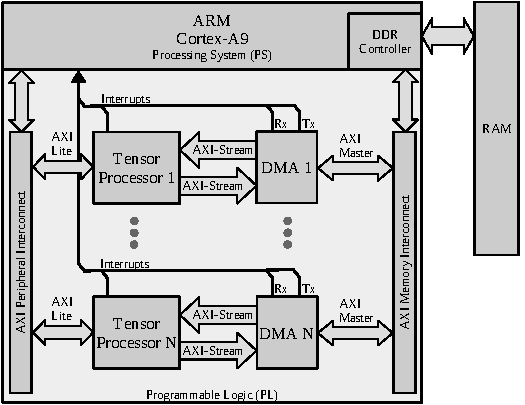
\includegraphics[width=0.5\columnwidth]{./chapters/cnn_accelerator/figures/system_design.pdf}
	\caption{Base embedded system architecture.}
	\label{fig:system_architecture}
\end{figure*}
\subsection{Tensor Processor}
The TP is a dedicated hardware module to compute tensor operations. This architecture implements high performance communication with AXI-Stream, direct CPU communication with AXI-Lite, and on-chip storage utilizing BRAM. This hardware architecture is implemented with high-level synthesis (HLS). The tensor operations are implemented based on the C++ TensorFlow Lite micro kernels. See \fig{fig:accelerator}.

The TP is an extensible hardware module that executes low-level tensor operations. In this paper, we focus on the \emph{Conv2D} tensor operation that computes 2D convolution layers.

\begin{figure*}[b!]
	\centering
	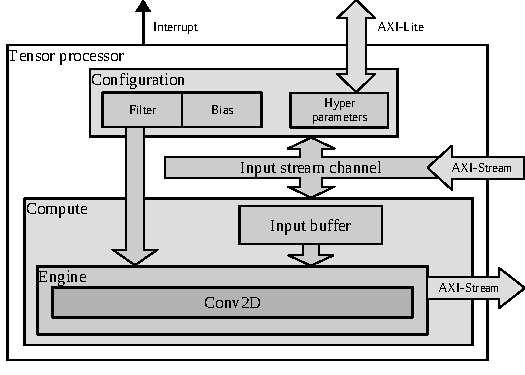
\includegraphics[width=0.5\columnwidth]{./chapters/cnn_accelerator/figures/accelerator.pdf}
	\caption{Hardware architecture of the proposed tensor processor.}
	\label{fig:accelerator}
\end{figure*}
\subsubsection{Modes of Operation}
The TP has two modes of operation: \emph{configuration} and \emph{execution}.
\begin{itemize}
	\item In \emph{configuration} mode, the TP receives the tensor operation hyperparameters: stride, dilation, padding, offset, activation, depth-multiplier, input shape, filter shape, bias shape, and output shape. Afterwards, the TP receives filter and bias tensors, which are locally stored in BRAM. The filter and bias tensors are transferred with standard FP representation. Then, the TP extracts the 6-bit FP format for local on-chip storage.
	
	\item In \emph{execution} mode, the TP executes the tensor operation according to the hyperparameters given in the configuration mode. During execution, the input and output tensors are moved from/to the off-chip memory via DMA.
\end{itemize}
\subsubsection{Dot-Product with Hybrid Floating-Point Computation}
\label{sec:dot_product}
We implement the floating-point computation adopting the dot-product with hybrid custom floating-point\cite{nevarez2021accelerating}. The hardware dot-product is illustrated in \Fig{fig:dot_product} and \Fig{fig:dot_product_loop}(a). This design instantiates an HF6 MAC and an accumulator variable of 64-bit fixed-point with 23-bit fraction. During operation, the feature map and filter values are extracted from on-chip memory (BRAM). Both values have to be different than zero to enable the MAC operation. The result is biased by accumulating a denormalized bias value. Since the bias is stored with 6-bit FP, its fractional part has to be aligned with the 23-bit fraction of the accumulator, see \Fig{fig:dot_product_loop}(b). The ReLu activation is applied and the result is normalized to converted to IEEE 754 standard FP, see \Fig{fig:dot_product_loop}(c).

Rather than a parallelized structure, this is a pipelined hardware design suitable for resource-limited devices. The latency in clock cycles of this hardware module is defined by \equ{eq:dot_custom_float_latency}, where $N$ is the vector length. This latency equation is obtained from the general pipelined hardware latency formula: $L=\left(N-1\right)II+IL$, where $II$ is the initiation interval, and $IL$ is the iteration latency. Both $II$ and $IL$ are obtained from the high-level synthesis results. Both the exponent and mantissa bit widths of the filter and bias buffers are set to a 4-bit exponent and a 1-bit mantissa (E4M1), which corresponds to float6 quantization.

\begin{eqnarray} \label{eq:dot_custom_float_latency}
L_{hf}=N+7
\end{eqnarray}

\begin{figure*}[b!]
	\centering
	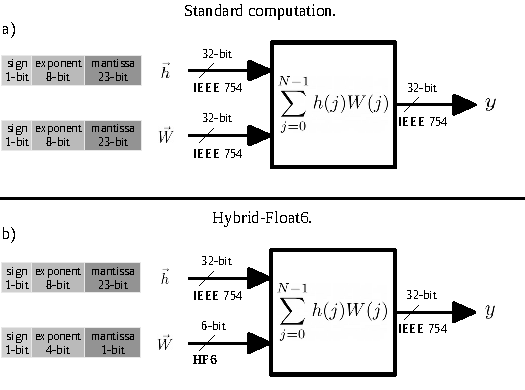
\includegraphics[width=0.5\columnwidth]{./chapters/cnn_accelerator/figures/dot-product_unit.pdf}
	\caption{Dot-product hardware module with (a) standard floating-point and (b) Hybrid-Float6.}
	\label{fig:dot_product}
\end{figure*}

\begin{figure*}[b!]
	\centering
	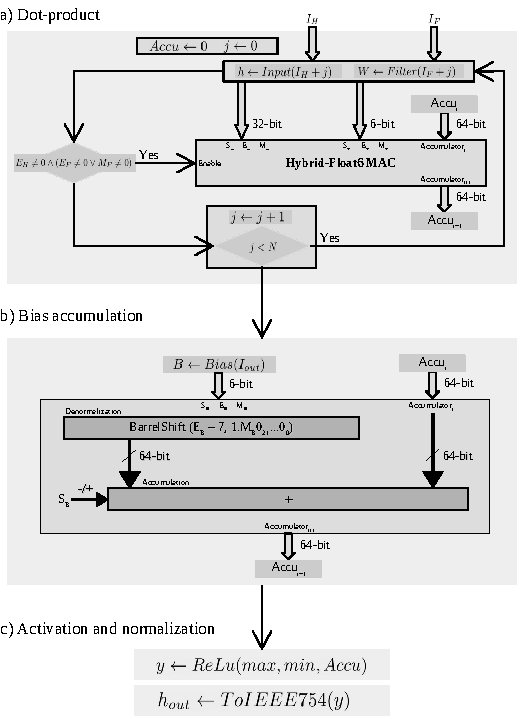
\includegraphics[width=0.5\columnwidth]{./chapters/cnn_accelerator/figures/dot_product_hybrid.pdf}
	\caption{(a) Dot-product hardware module with Hybrid-Float6 MAC, (b) bias accumulation, (c) activation and normalization.}
	\label{fig:dot_product_loop}
\end{figure*}

\subsubsection{Multiply-Accumulate}
The multiply-accumulate operation calculates the product of two numbers and adds the result to an accumulator. In FP arithmetics, the size of a hardware multiplier scales with the size of the mantissas. In the case of HF6, the 6-bit FP representation allows optimization in the mantissa multiplication. The 1-bit mantissa enables efficient MAC implementations by reducing the mantissa multiplication to a multiplexed addition, see \fig{fig:multiplier}. The denormalized results are accumulated in a fixed-point accumulator. This approach reduces latency, energy consumption, and resource utilization.

\begin{figure*}[b!]
	\centering
	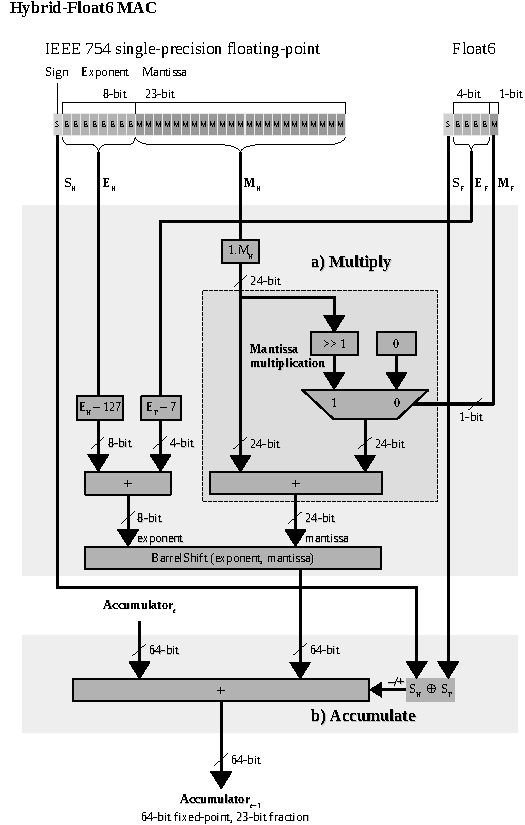
\includegraphics[width=0.5\columnwidth]{./chapters/cnn_accelerator/figures/multiplier.pdf}
	\caption{Hybrid-Float6 multiply-accumulate hardware design.}
	\label{fig:multiplier}
\end{figure*}

The Infinity and NaN special cases are not considered in this design since are not expected in ANN computation. For the subnormal case, the element-wise multiplication is disabled when having a zero entry and is approximated when having subnormal mantissa. The feature map values are considered zero when the exponent is zero ($E_H=0$). The filter values are considered zero when both exponent and mantissa are zero ($E_F=0\land M_F=0$). See \Fig{fig:dot_product_loop}(a). In the 6-bit FP, the 1-bit mantissa has one subnormal case, which is handled as a normalized case. This exploits the intrinsic error tolerance of ANN to reduce the hardware design.

The approximation error is defined by the difference between \Equ{eq:float} and \Equ{eq:float_subnorm} when $E=0$ and $M=2^{-1}$. The result defines the error as $e=2^{-B-1}$. Then, from \Equ{eq:float_bias} with $E_{size}=4$, we have $B=7$. Hence, $e=3.9\mathrm{e}{-3}$. This error is produced when having the subnormal case $E=0$ and $M=2^{-1}$, which corresponds to the value $\pm7.8\mathrm{e}{-3}$ deviated to $\pm1.17\mathrm{e}{-2}$. This approximation leverages the intrinsic error tolerance of ANN to reduce hardware resource utilization and energy consumption \cite{du2014leveraging}.


\subsubsection{On-Chip Memory Utilization}
\label{sec:memory_utilization}
The total on-chip memory utilization on the TP is defined by \Equ{eq:tp_memory}, where $TP_B$ and $V_{M}$ represent the tensor buffers and local variables (memory) required for the design, respectively. \Equ{eq:tp_memory_buffer} defines the tensor buffers, where $Input_{M}$ is the \emph{input buffer}, $Filter_{M}$ is the \emph{filter buffer}, $Bias_{M}$ is the \emph{bias buffer}. The on-chip memory buffers are defined in bits. \fig{fig:accelerator_buffers} illustrates the convolution operation utilizing the on-chip memory buffers.
\begin{figure*}[b!]
	\centering
	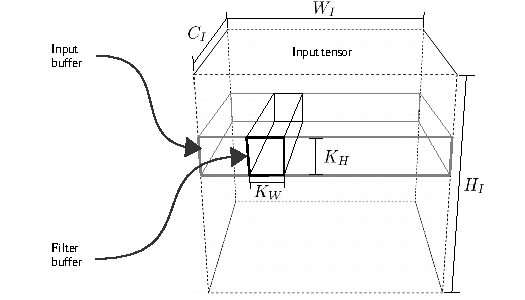
\includegraphics[width=0.5\columnwidth]{./chapters/cnn_accelerator/figures/accelerator_buffers.pdf}
	\caption{Design parameters for on-chip memory buffers on the TP.}
	\label{fig:accelerator_buffers}
\end{figure*}
\begin{eqnarray} \label{eq:tp_memory}
TP_{M}=TP_B+V_{M}
\end{eqnarray}
\begin{eqnarray} \label{eq:tp_memory_buffer}
TP_{B}=Input_{M}+Filter_{M}+Bias_{M}
\end{eqnarray}

The memory utilization of \emph{input buffer} is defined by \Equ{eq:input_memory}, where $K_{H}$ is the height of the convolution kernel, $W_{I}$ is the width of the input tensor, $C_{I}$ is the number of input channels, and $BitSize_{I}$ is the bit size of input tensor.
\begin{eqnarray} \label{eq:input_memory}
Input_{M}=K_{H}W_{I}C_{I}BitSize_{I}
\end{eqnarray}

The memory utilization of \emph{filter buffer} is defined by \Equ{eq:filter_memory}, where $K_{W}$ and $K_{H}$ are the width and height of the convolution kernel, respectively; $C_{I}$ and $C_{O}$ are the number of input and output channels, respectively; and $BitSize_{F}$ is the bit size of filter values.
\begin{eqnarray} \label{eq:filter_memory}
Filter_{M}=C_{I}K_{W}K_{H}C_{O}BitSize_{F}
\end{eqnarray}

The memory utilization of \emph{bias buffer} is defined by \Equ{eq:bias_memory}, where $C_{O}$ is the number of output channels, and $BitSize_{B}$ is the bit size of bias values.
\begin{eqnarray} \label{eq:bias_memory}
Bias_{M}=C_{O}BitSize_{B}
\end{eqnarray}

As a design trade-off, \Equ{eq:channel_in_memory} defines the capacity of output channels based on the given design parameters. The total on-chip memory $TP_{M}$ determines the TP capacity.
\begin{eqnarray} \label{eq:channel_in_memory}
C_{O}=\frac{TP_{M}-V_{M}-K_{H}W_{I}C_{I}BitSize_{I}}{C_{I}K_{W}K_{H}BitSize_{F}+BitSize_{B}}
\end{eqnarray}

The floating-point formats implemented in the TP are defined by $BitSize_F$, $BitSize_B$ and $BitSize_I$. The HF6 defines 6-bit for $BitSize_F$ and $BitSize_B$, and 32-bit for $BitSize_I$. These are design parameters defined before hardware synthesis. This allows fine control of BRAM utilization, which is suitable for resource-limited devices.

\subsection{Training Method}
The models are trained and quantized in separate stages.
\subsubsection{Training with Iterative Early Stop}
To achieve better performance on CNN-regression models, we implement a training procedure with iterative early stop cycle. This allows to reach better local minima. This is a four steps process:

\begin{enumerate}
	\item A model is obtained with an initial training with standard early stop monitoring.
	\item The model is iteratively re-trained with standard early stop to search for better local minima. In each early stop the Adam optimizer restarts the moving averages.
	\item In case of a better local minimum, the base model is updated/saved and used for subsequent re-training iterations, otherwise it is discarded.
	\item The cyclic process stops automatically with a given patience. This allows to set a maximum training iterations before the stop.
\end{enumerate}

This method is described in \Algo{alg:training}.

\subsubsection{Quantization Aware Training}
The quantization aware training (QAT) method is integrated into the training process, this operates after each mini-batch update. The quantization is applied on the trainable parameters of convolution layers. This method is implemented as a callback function in the TensorFlow/Keras framework, see \Algo{alg:quantization_integration}.

The quantization method uses rounding strategy to reduce the FP representation. This maps the full precision FP values to the closest representable 6-bit FP values, see \Algo{alg:quantize_training}. This method quantizes the filter and bias tensors of the convolution layers. We have observed that the exponent bit size plays a more predominant influence on the model accuracy than the mantissa bit size. In \cite{lai2017deep}, Lai et al. demonstrated that 4-bit exponent is adequate and consistent across different networks (SqueezeNet, AlexNet, GoogLeNet, VGG-16). In this work, we investigate 4-bit exponent and 1-bit mantissa.

\begin{algorithm}[h!]
	\caption{Training with iterative early stop cycle.}
	\label{alg:training}
	\begin{algorithmic}
		\SetAlgoLined
		\renewcommand{\algorithmicrequire}{\textbf{input:}}
		\renewcommand{\algorithmicensure}{\textbf{output:}}
		\REQUIRE $MODEL$ as the input model.
		\REQUIRE $D_{train}$ as the training data set.
		\REQUIRE $D_{val}$ as the validation data set.
		\REQUIRE $N_{I}$ as the stop patience for iterative training cycle.
		\REQUIRE $N_{E}$ as the early stop patience (epochs) for training.
		\REQUIRE $B_{size}$ as the mini-batch size.
		\ENSURE $MODEL$ as the full-precision output model.
		\STATE $Train(MODEL, D_{train}, D_{val}, N_{E}, B_{size})$
		\STATE $mse_i \gets Evaluate(MODEL, D_{val})$ // Benchmark
		\STATE $n_i \gets 0$
		\WHILE {$n_i<N_I$}
		\STATE // Iterative early stop cycle
		\STATE $Train(MODEL, D_{train}, D_{val}, N_{E}, B_{size})$
		\STATE $mse_v \gets Evaluate(MODEL, D_{val})$
		\IF{$mse_v < mse_i$}
		\STATE $Update(MODEL)$
		\STATE $mse_i \gets mse_v$
		\ELSE
		\STATE $MODEL  \gets LoadPreviousModel()$
		\STATE $n_I \gets n_I + 1$
		\ENDIF
		\ENDWHILE
	\end{algorithmic}
\end{algorithm}


\begin{algorithm}[h!]
	\caption{OnMiniBatchUpdate\_Callback.}
	\label{alg:quantization_integration}
	\begin{algorithmic}
		\SetAlgoLined
		\renewcommand{\algorithmicrequire}{\textbf{input:}}
		\renewcommand{\algorithmicensure}{\textbf{output:}}
		\REQUIRE $MODEL$ as the full-precision input model.
		\REQUIRE $E_{size}$ as the target exponent bits size.
		\REQUIRE $M_{size}$ as the target mantissa bits size.
		\REQUIRE $D_{train}$ as the training data set.
		\REQUIRE $D_{val}$ as the validation data set.
		\REQUIRE $N_{ep}$ as the number of epochs.
		\REQUIRE $B_{size}$ as the mini-batch size.
		\ENSURE $MODEL$ as the quantized output model.
		\STATE //Quantize
		\STATE $MODEL \gets \Algo{alg:quantize_training}(MODEL,E_{size}, M_{size})$ 
		\IF {$1<epoch$}
		\STATE // Update model after first epoch
		\STATE $mse_v \gets Evaluate(MODEL, D_{val})$
		\IF{$mse_v < mse_i$}
		\STATE $Update(MODEL)$
		\STATE $mse_i \gets mse_v$
		\ENDIF
		\ENDIF
	\end{algorithmic}
\end{algorithm}

\begin{algorithm}[h!]
	\caption{Custom floating-point quantization.}
	\label{alg:quantize_training}
	\begin{algorithmic}
		\SetAlgoLined
		\renewcommand{\algorithmicrequire}{\textbf{input:}}
		\renewcommand{\algorithmicensure}{\textbf{output:}}
		\REQUIRE $MODEL$ as the CNN.
		\REQUIRE $E_{size}$ as the target exponent bit size.
		\REQUIRE $M_{size}$ as the target mantissa bits size.
		\REQUIRE $STDM_{size}$ as the IEEE 754 mantissa bit size.
		\ENSURE $MODEL$ as the quantized CNN.
		\FOR {$layer$ in $MODEL$}
		\IF {$layer$ is $Conv2D$ or $SeparableConv2D$}
		\STATE $filter, bias \gets GetWeights(layer)$
		\FOR {$x$ in $filter$ and $bias$}
			\STATE $sign \gets GetSign(x)$
			\STATE $exp \gets GetExponent(x)$
			\STATE $fullexp \gets 2^{E_{size}-1}-1$ // Get full range value
			\STATE $cman \gets GetCustomMantissa(x, M_{size})$
			\STATE $leftman \gets GetLeftoverMantissa(x, M_{size})$
			\IF {$exp <-fullexp$}
				\STATE$x\gets0$
			\ELSIF{$exp > fullexp$}
				\STATE$x\gets (-1)^{sign}\cdot2^{fullexp}\cdot(1+(1-2^{-M{size}}))$
			\ELSE
				\IF {$2^{STDM_{size}-M_{size}-1}-1<leftman$}
					\STATE $cman \gets cman+1$ // Above halfway
					\IF{$2^{M_{size}}-1<cman$}
					\STATE $cman \gets 0$ // Correct mantissa overflow
					\STATE $exp \gets exp + 1$
					\ENDIF
				\ENDIF
				\STATE // Build custom quantized floating-point value
				\STATE$x\gets (-1)^{sign}\cdot2^{exp}\cdot(1+cman\cdot2^{-M_{size}})$
			\ENDIF
		\ENDFOR
		\STATE $SetWeights(layer, filter, bias)$
		\ENDIF
		\ENDFOR
	\end{algorithmic}
\end{algorithm}
\begin{figure*}[b!]
	\centering
	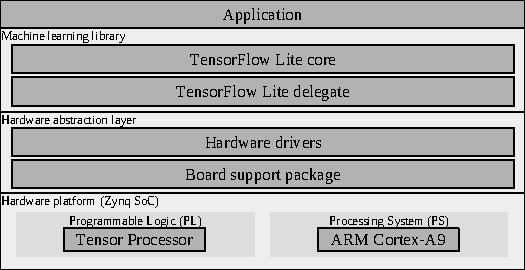
\includegraphics[width=0.5\columnwidth]{./chapters/cnn_accelerator/figures/sw_stack.pdf}
	\caption{Base embedded software architecture.}
	\label{fig:sw_stack}
\end{figure*}
\subsection{Embedded software architecture}
The software architecture is a layered object-oriented application framework written in C++, see \fig{fig:sw_stack}. A description of the software layers is as follows:
\begin{itemize}
	\item \emph{Application}: As the highest level of abstraction, this software layer implements the application invoking the ML library.
	\item \emph{Machine learning library}: This layer consist of TensorFlow Lite for micro controllers. This offers a comprehensive high level API that allows ML inference. This provides delegate software interfaces for custom hardware accelerators.
	\item \emph{Hardware abstraction layer}: This layer consist of the hardware drivers to handle initialization and runtime operation of the TP and DMA.
\end{itemize}
\section{Experimental Results}
\label{sec:experimental_results}
This section presents experimental results using a low-power/low-cost sensor analytics application. A \gls{cnn}-regression model is proposed to predict x- y- coordinates of acoustic emissions based on piezoelectric vibrations. Quantitative and qualitative aspects of the analytics are compared using floating-point 32-bit, fixed-point 8-bit, Hybrid-Logarithmic 6-bit, and Hybrid-Float6.

To demonstrate the proposed concept, the \gls{cnn} model is deployed in the smallest Zynq \gls{soc} \gls{fpga} device for low-power inference. The performance of the \gls{tp} synthesized with standard \gls{fp} (using Xilinx LogiCORE IPs) and Hybrid-Float6 design.

\subsection{Sensor Analytics Application}
The analytics model is designed to predict x- y- coordinates of acoustic emissions on a metal plate. The metal plate is in the presence of noise disturbance to simulate realistic conditions. This subsection presents the structure for experimental setup, data sets, and the \gls{cnn}-regression model.

\subsubsection{Experimental Setup}
The experiment uses eight piezoelectric sensors (Vallen Systeme VS900) attached with magnetic holders on a metal plate ($\unit[90]{cm}\times\unit[86.6]{cm}\times\unit[0.3]{cm}$). The VS900 devices can operate either in active or passive mode. Six VS900 are used in passive mode as acoustic sensors and two in active mode to produce acoustic emissions. These acoustic emissions simulate anomalies on x- y- coordinates as well as the noise disturbance on the system. See \fig{fig:data_set}(a). To create data sets, the samples of acoustic emissions are labeled with their coordinates.

\subsubsection{Data Sets}
The data sets are recorded applying pulses on the metal plate, the x- y- coordinates of these pulses are used as labels. The pulses for training and validation data sets are shown in \fig{fig:data_set}(b) and \fig{fig:data_set}(c), respectively. The pulses for training and validation data sets are mutually exclusive, this exclusion is represented by the cross symbols in \fig{fig:data_set}(c). This creates a grid layout used to collect samples for the data sets. This grid is $10\times10$ divisions, these are on the metal plate area ($\unit[90]{cm}\times\unit[86.6]{cm}$). This grid does not consider the four corners as they are used for magnetic holders.

\begin{figure}[t!]
	\centering
	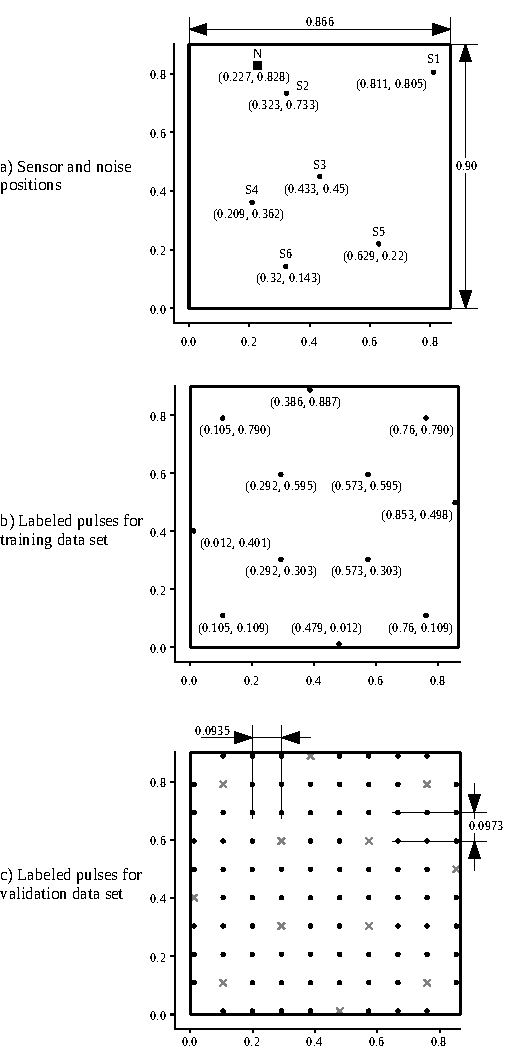
\includegraphics[width=0.5\textwidth]{./chapters/cnn_accelerator/figures/histograms/data_set.pdf}
	\caption{Experimental setup for sensor analytics on structural health monitoring, all lengths are in meters (m).}
	\label{fig:data_set}
\end{figure}

In order to create reproducible acoustic emissions, this demonstration uses 9-cycle sine pulse in a Hanning window with central frequency $f_\mathrm{c}$ (narrow-banded in the frequency domain). This experiment assumes guided Lamb waves based on the plate structure. The narrow-band behavior also reduces the dispersion of the acoustic emission waves~\cite{hannwindowsine}. The waveform can be expressed as a function of time $t$ as follows:

\begin{equation}
x_\mathrm{pulse}(t) = \frac{1}{2} \Big(1-\cos{\frac{f_\mathrm{c} t}{5}} \Big) A_0 \sin{f_\mathrm{c} t}.
\end{equation}

To generate the data sets, slightly different pulse amplitudes and frequencies for excitation are used. The pulse frequency $f_c$ is varied in $\unit[1]{kHz}$ steps between $\unit[300]{kHz}$ and $\unit[349]{kHz}$ and the amplitude $A_0$ is varied in $\unit[0.1]{V}$ steps between $\unit[2.6]{V}$ and $\unit[3.5]{V}$. This produces 500 different pulses for each of the excitation points.

The signals for labeled pulses and noise disturbance are generated by \glspl{awg}. The sensor signals are recorded via a Vallen AMSY-6 measurement system with a resolution of 18 bits and a sampling rate of $f_\mathrm{S} =\unit[10]{MHz}$. The disturbance signal is gaussian noise with amplitudes between 0-3 V. This noise is applied via the piezoelectric device $N$ at $x=\unit[0.227]{m}$ and $y=\unit[0.828]{m}$, see \fig{fig:data_set}(a).

To obtain frequency components, the sampled pulses are converted into the frequency-time domain using the \gls{stft}. This is calculated as follows~\cite{stft_lit}:

\begin{flalign}
\label{stft_eq2}
\mathcal{F}_{m,k}^\gamma= \sum_{n=0}^{N-1} x[n] \cdot \gamma^*[n-m\Delta M]\cdot \mathrm{e}^{\frac{-j 2 \pi k n }{N}}
\end{flalign}

Here $x[n]$ describes a discrete-time signal and $\gamma^*[n-m\Delta M]\cdot \mathrm{e}^{\frac{-j 2 \pi k n }{N}}$ the time- and frequency-shifted window function inside the considered interval $[0 , N-1]$. $\Delta M$ describes the time shift and $N$ the transformation window. Since only discrete frequencies and time points are considered, $m = 0,1,...,M-1$ is valid. For pictorial representation, the magnitude of the complex-valued \gls{stft} is employed in a spectrogram $\mathcal{S}_{m,k}$:

\begin{flalign}
\label{stft_eq3}
\mathcal{S}_{m,k}= \left|\mathcal{F}_{m,k}^\gamma\right|^2 = \left|\sum_{n=0}^{N-1} x[n] \cdot \gamma^*[n-m\Delta M]\cdot \mathrm{e}^{\frac{-j 2 \pi k n }{N}} \right|^2
\end{flalign}

In addition, these spectrograms are scaled in decibels. The spectrogram in decibels $\mathcal{S}_{m,k,\mathrm{dB}}$ produces $\mathcal{S}_{m,k,\mathrm{dB}}= 20 \cdot \mathrm{log}_{10}(\mathcal{S}_{m,k})$. For conversion of data, the experiment uses a signal length of 400 \textmu s (75 \textmu s pretrigger and 325 \textmu s post trigger). Thus, the arrival times of the pulses are included in the spectrogram for all channels and labeled positions. This uses Blackman window function~\cite{blackman_window}, \gls{fft} length of 32 samples, and overlap of 8 samples. The spectrograms are calculated for frequencies in the range of \unit[100]{kHz} to \unit[500]{kHz}. This produces a spectrogram size of 8x16 (8 frequency bins, 16 time values).

In order to generate larger data sets, four further variants are created with time shifts of 15 \textmu s/ 30 \textmu s/ 45 \textmu s/ 60 \textmu s. Subsequently, all spectrograms are converted to grayscale with scaling between \unit[-100]{dB} and \unit[-40]{dB}, see \fig{fig:spectrograms}.

In overall, the data set has a size of 1,440,000 images. This is the result of 500 (pulses) $\cdot$ 5 (spectrograms) $\cdot$ 6 (listening sensors) $\cdot$ 96 (excitation points).

\begin{figure}[t!]
	\centering
	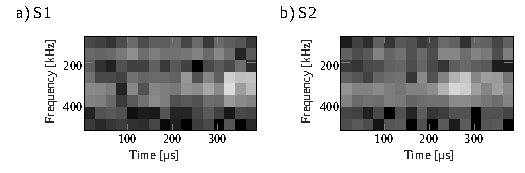
\includegraphics[width=0.5\textwidth]{./chapters/cnn_accelerator/figures/histograms/spectrograms.pdf}
	\caption{Spectrograms of sensors $S_1, S_2$ converted to grayscale for pulses at $x =0.105$ m, $y = 0.109$ m with noise disturbance.}
	\label{fig:spectrograms}
\end{figure}

\subsubsection{CNN-Regression Model}
The data analytics is implemented with a \gls{cnn}-regression model, see \fig{fig:model}. The structure of the model is described below:

\begin{enumerate}[label=\alph*)]
\item Input tensor. This is composed of spectrograms from the sensor signals. The tensor shape is defined by $S \times T \times F$, where $S$ is the number of sensors, and $T \times F$ is the time-frequency resolution of the spectrograms, see \fig{fig:model}(a).

\item Feature extraction. This is composed of three blocks of convolution, batch normalization, and max-pooling layers, see \fig{fig:model}(b). The number of channels in the convolution layers are defined by the hyper-parameters $A$, $B$, and $C$.

\item Regression function. This is an arbitrary function implemented with two fully connected layers and an output layer with linear activation, see \fig{fig:model}(c).
\end{enumerate}


\begin{figure}[t!]
	\centering
	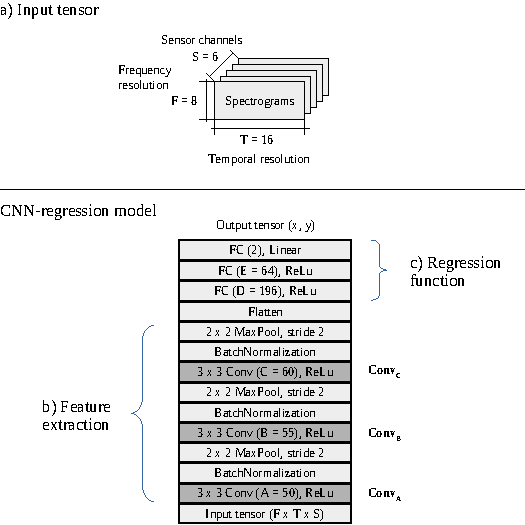
\includegraphics[width=0.5\textwidth]{./chapters/cnn_accelerator/figures/models.pdf}
	\caption{CNN-regression model for sensor analytics.}
	\label{fig:model}
\end{figure}


\subsection{Training}
\subsubsection{Base Model}
The model in \fig{fig:model} is trained using Adam algorithm with iterative search. The Adam optimizer is configured with the default settings presented in \cite{kingma2014adam}: $\alpha = 0.001$, $\beta_1 = 0.9$, $\beta_2 = 0.999$, and $\epsilon = 1\mathrm{e}{-8}$. The training-cycle has a patience of 10 iterations before stop, the optimizer is executed with early stop patience of 10 epochs, and mini-batch size of 512 samples. This is applied using the method described in \Algo{alg:training} with $N_I = 10$, $N_E=10$, $B_{size}=512$.

The training results are illustrated in \fig{fig:optimization}(a). In this optimization, the initial and the final models achieve $MSE=\unit[0.0135]{m^2}$ and $MSE=\unit[0.0122]{m^2}$, respectively. The $MSE$ is calculated with the Euclidean distance (loss) between the real/expected and the predicted/inferred coordinates. The initial model is obtained at the first early stop (after 10 epochs). In each stop, the moving averages of the Adam optimizer get re-initialized. This facilitates searching for better local minima. The model gets saved/updated when finding a better minimum.

\begin{figure}[h!]
	\centering
	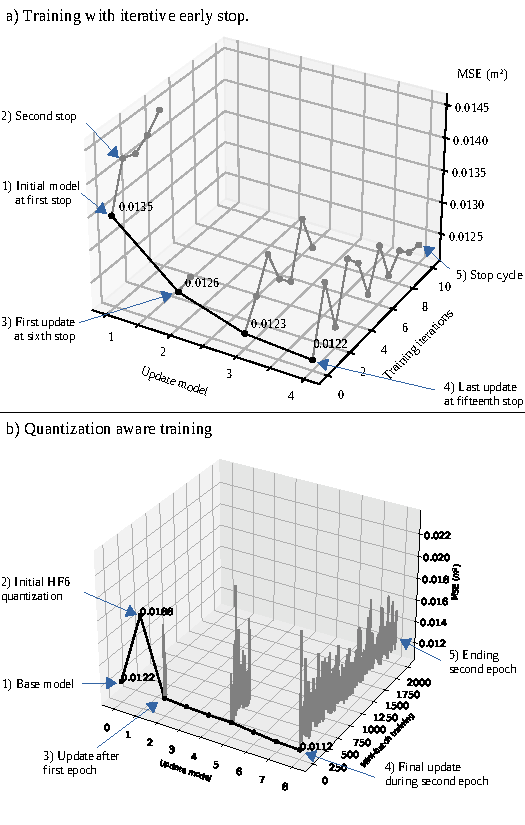
\includegraphics[width=0.5\textwidth]{./chapters/cnn_accelerator/figures/histograms/training_and_quantization.pdf}
	\caption{Training results.}
	\label{fig:optimization}
\end{figure}

The final model achieves $MSE=\unit[0.0122]{m^2}$, which corresponds to $MAE=\unit[0.0955]{m}$. See \fig{fig:model_evaluation}(a). In total, the training takes 379 epochs in 25 cycle-search iterations. The first search takes 43 epochs for the initial model and subsequent search iterations take an average of 14 epochs. The total time is 53 minutes using a \gls{pc} with AMD Ryzen 5 5600H and NVIDIA GeForce RTX 3050 \gls{gpu}.

\begin{figure}[h!]
	\centering
	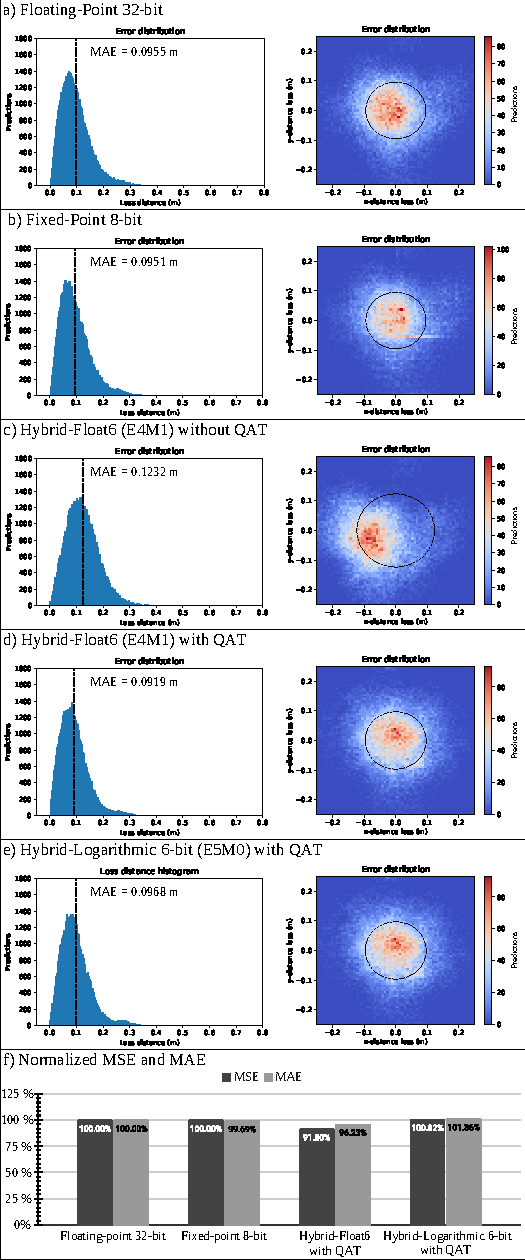
\includegraphics[width=0.5\textwidth]{./chapters/cnn_accelerator/figures/histograms/model_evaluation.pdf}
	\caption{Performance of the model with different data representations.}
	\label{fig:model_evaluation}
\end{figure}

\subsubsection{TensorFlow Lite 8-bit Quantization}
This optimization method converts filter and bias tensors as well as activation maps to 8-bit integer representation, this allows inference using integer-only arithmetic~\cite{hannwindowsine}. In this research, this quantization is applied only to the convolution layers as they are the compute bound operations. Other layers employ 32-bit \gls{fp} representation.

In the compute graph, the input and output feature maps are glued with linear quantization at the input and output of the \emph{Conv2D} operations.

The base model is quantized using the TensorFlow Lite library with integer-only quantization on the \emph{Conv2D} tensor operations. The filter and bias tensors are represented by 8-bit and 32-bit signed integers, respectively. The input and output activation maps are represented by 8-bit signed integer. The TensorFlow quantization includes two additional vectors (output-multiplier and output-shift coefficients), these two vectors are the same shape as the bias vector with 32-bit integer representation.

This model achieves $MSE=\unit[0.0126]{m^2}$ and $MAE=\unit[0.0992]{m}$. See \fig{fig:model_evaluation}(b). The MAE increases 5.1\% of the base model. We attribute this degradation to the 8-bit quantization on the \emph{Conv2D} layers.

\subsubsection{Inference of non-quantized models on HF6 hardware}
To demonstrate backward compatibility, the inference quality of the base model is measured without quantization on the \gls{hf6} hardware. See \fig{fig:model_evaluation}(c). This obtains $MSE=\unit[0.0188]{m^2}$ and $MAE=\unit[0.1232]{m}$. The MAE increases 29.5\% of the base model. We attribute this degradation to the rounding errors of non-quantized filters and bias in \emph{Conv2D} layers.

\subsubsection{Quantization-Aware Training for HF6 hardware}
The \gls{qat} is a post-training optimization. This has been run during two epochs with mini-batch size of 10 samples. This quantization is executed targeting the HF6 format: 4-bit exponent and 1-bit mantissa. This is applied to filter and bias tensors of \emph{Conv2D} layers. This method is described in \Algo{alg:quantization_integration} with $N_{ep}=2$, $B_{size}=10$, $E_{size}=4$, $M_{size}=1$. The optimization results are illustrated in \fig{fig:optimization}(b).

The resulting model achieves $MSE=\unit[0.0112]{m^2}$ and $MAE=\unit[0.0919]{m}$. This corresponds to an error reduction of 8.2\% and 3.77\%, respectively. We attribute this improvement to the regularization effect. See \fig{fig:model_evaluation}(d). The \gls{qat} time is 185 minutes.


\subsubsection{Quantization-Aware Training for Hybrid-Logarithmic 6-bit}
For the sake of quality comparison with logarithmic quantization, the model with 6-bit logarithmic representation is generated. See \fig{fig:floating}(e). This quantization matches the bit size of \gls{hf6}. The filter and bias tensors of \emph{Conv2D} layers are quantized with the 6-bit logarithmic format: 1-bit sign, 5-bit signed exponent, and 0-bit mantissa. This is applied using the method described in \Algo{alg:quantization_integration} with $N_{ep}=2$, $B_{size}=10$, $E_{size}=5$, $M_{size}=0$.

The model achieves $MSE=\unit[0.0123]{m^2}$ and $MAE=\unit[0.0968]{m}$, which correspond to an error increase of 0.82\% and 1.36\%, respectively. We attribute this degradation to the 6-bit logarithmic quantization lacking fractional bits. See \fig{fig:model_evaluation}(e).

A summary of improvement-degradation of MSE and MAE with different data representations is presented in \fig{fig:model_evaluation}(f).

\subsection{Hardware Design Exploration}
The proposed hardware/software co-design is demonstrated on the Zynq-7007S \gls{soc} on the MiniZed development board. This \gls{soc} integrates a single ARM Cortex-A9 \gls{ps} and a \gls{pl} equivalent to Xilinx Artix-7 \gls{fpga} in a single chip~\cite{xilinx2015zynq}. The Zynq-7007S \gls{soc} architecture maps the custom logic and software in the \gls{pl} and \gls{ps}, respectively.

In this platform, the proposed hardware/software architecture is implemented to deploy the sensor analytics application. The desired model is converted to TensorFlow Lite (floating-point) and deployed on the embedded software as a hex dump as a C array. The Zynq-7007S \gls{soc} executes inference with TensorFlow Lite on the \gls{ps}. The computational workload of convolution layers is delegated to the dedicated hardware.

\subsubsection{Benchmark on Embedded CPU}
First, the performance of the embedded \gls{cpu} is explored for inference without hardware acceleration. In this case, TensorFlow Lite creates the \gls{cnn} model as a sequential compute graph executing all computation on the \gls{cpu} (ARM Cortex-A9) at $\unit[666]{MHz}$ with power dissipation of $\unit[1,187]{W}$.

The compute performance and run-time inference of the \gls{cpu} are shown in \Tab{tab:performance}(a) and \fig{fig:runtime}(a), respectively.

\subsubsection{Benchmark on Tensor Processor Synthesized with Xilinx LogiCORE IP for Floating-Point Computation}
For this design, the TP is implemented with standard Xilinx \gls{fp} hardware prior synthesis. The design parameters for the maximum required accelerator on-chip size are:
\begin{itemize}
	\item Max convolution kernel size: $K_W = K_H = 3$.
	\item Max input tensor width: $W_I = 16$.
	\item Max input and output channels: $C_I = 55$, $C_O = 60$.
	\item Filter and bias bit size: $BitSize_F=BitSize_B=32$.
	\item Input tensor bit size: $BitSize_I=32$.
\end{itemize}

Using equations from Section \ref{sec:memory_utilization}, the on-chip memory utilization are $Input_M=84,480$b, $Filter_M=950,400$b, and $Bias_M=1,920$b. Hence, the required on-chip memory buffer size is $TP_B=1,036,800$b.

The post-implementation resource utilization and power dissipation are presented in \Tab{tab:resource_utilization}(a). The complete hardware platform utilizes 83\% of BRAM, this includes the on-chip memory requirements of the \gls{tp}, \gls{dma}, and AXI interconnects. The total available on-chip memory (BRAM) on the Zynq-7007S \gls{soc} is $\unit[1.8]{Mb}$. After hardware syntheses, the estimated power dissipation of the \gls{tp} is $\unit[85]{mW}$ at $\unit[200]{MHz}$ (this estimation is provided by Xilinx Vivado).

\begin{table}[!h]\centering
	\caption{Resource utilization and power dissipation on the Zynq-7007S SoC.}\label{tab:resource_utilization}
	\scriptsize
	\begin{tabular}{lrrrrrr}\toprule
		\multirow{2}{*}{\textbf{TP engine}} &\multicolumn{4}{c}{\textbf{Post-implementation resource utilization}} &\multirow{2}{*}{\textbf{Power (W)}} \\\cmidrule{2-5}
		&\textbf{LUT} &\textbf{FF} &\textbf{DSP} &\textbf{BRAM 36Kb} & \\\midrule
		\multirow{2}{*}{(a) Floating-Point} &5,578 &8,942 &23 &41.5 &\multirow{2}{*}{1.429} \\
		&39\% &31\% &35\% &\textbf{83\%} & \\
		\multirow{2}{*}{(b) Hybrid-Float6} &7,313 &10,330 &20 &15 &\multirow{2}{*}{1.424} \\
		&51\% &36\% &30\% &\textbf{30\%} & \\
		\bottomrule
	\end{tabular}
\end{table}

The compute performance and inference schedule of the model on this hardware implementation are shown in \Tab{tab:performance}(b) and \fig{fig:runtime}(b), respectively. During run-time, the software (TensorFlow Lite) delegates computation to the \gls{tp} as dedicated hardware for \emph{Conv2D} tensor operations.

The implementation of the dot-product with standard \gls{fp} engine (IEEE 754 arithmetic) utilizes proprietary multiplier and adder floating-point operator cores. Vivado \gls{hls} implements \gls{fp} arithmetic operations by mapping them onto Xilinx LogiCORE IP cores, these \gls{fp} operator cores are instantiated in the resultant \gls{rtl}~\cite{hrica2012floating}. In this case, the implementation of the dot-product with the standard \gls{fp} computation reuses the multiplier and adder cores in different compute sections of the \gls{tp}. The post-implementation resource utilization and power dissipation of the individual floating-point operator cores are shown in \Tab{tab:LogiCORE}.

\begin{table}[!t]\centering
	\caption{Compute performance of the CPU and TP on each Conv2D tensor operation. This table presents: tensor operation, computational cost in mega floating-point operations (MFLOP), latency, throughput, power efficiency, and estimated energy consumption as the energy delay product (EDP).}\label{tab:performance}
	\scriptsize
	\begin{tabular}{lrrrrrr}\toprule
		\textbf{Operation} &\textbf{MFLOP} &\textbf{t (ms)} &\textbf{MFLOP/s} &\textbf{MFLOP/s/W} &\textbf{EDP (mJ)} \\\midrule
		& &\multicolumn{4}{l}{\textbf{a) CPU (ARM Cortex-A9) @666MHz, 1.187 W}} \\
		Conv\textsubscript{A} &0.691 &112.24 &6.16 &5.19 &133.23 \\
		Conv\textsubscript{B} &1.584 &213.13 &7.43 &6.26 &252.99 \\
		Conv\textsubscript{C} &0.475 &46.59 &10.20 &8.59 &55.31 \\
		& &\multicolumn{4}{l}{\textbf{b) TP (Floating-Point engine) @200MHz, 85 mW}} \\
		Conv\textsubscript{A} &0.691 &12.49 &55.34 &651.11 &1.06 \\
		Conv\textsubscript{B} &1.584 &16.39 &96.66 &1,137.20 &1.39 \\
		Conv\textsubscript{C} &0.475 &3.59 &132.44 &1,558.13 &0.30 \\
		& &\multicolumn{4}{l}{\textbf{c) TP (Hybrid-Float6 engine) @200MHz, 84 mW}} \\
		Conv\textsubscript{A} &0.691 &6.92 &99.81 &1,188.24 &0.58 \\
		Conv\textsubscript{B} &1.584 &4.41 &358.94 &4,273.09 &0.37 \\
		Conv\textsubscript{C} &0.475 &0.99 &482.44 &5,743.29 &0.08 \\
		\bottomrule
	\end{tabular}
\end{table}

\begin{figure}[t!]
	\centering
	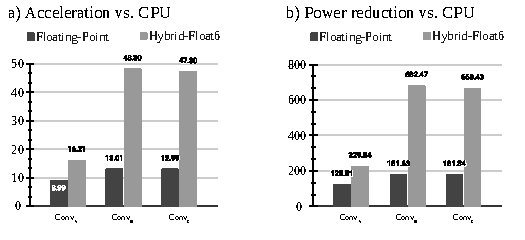
\includegraphics[width=0.5\textwidth]{./chapters/cnn_accelerator/figures/power_breakdown/acceleration_power_reduction.pdf}
	\caption{Inference acceleration and power reduction on the TP with floating-point and HF6 vs. CPU on the Zynq-7007S SoC.}
	\label{fig:acceleration}
\end{figure}


\begin{table}[!h]\centering
	\caption{Resource utilization and power dissipation of individual multiplier and adder floating-point (IEEE 754) operator cores (Xilinx LogiCORE IP).}\label{tab:LogiCORE}
	\scriptsize
	\begin{tabular}{lrrrrrr}\toprule
		\textbf{Core operation} &\textbf{DSP} &\textbf{FF} &\textbf{LUT} &\textbf{Latency (clk)} &\textbf{Power (mW)} \\\midrule
		Multiplier &3 &151 &325 &4 &7 \\
		Adder &2 &324 &424 &8 &6 \\
		\bottomrule
	\end{tabular}
\end{table}



\subsubsection{Tensor Processor Synthesized with Hybrid-Float6 Hardware Architecture}
To demonstrate the proposed design, the \gls{tp} with \gls{hf6} hardware reuses the standard \gls{fp} design parameters with the following variation for the 6-bit representation in filter and bias: $BitSize_F=BitSize_B=6$.

Using equations from Section \ref{sec:memory_utilization}, the on-chip memory requirements for the hardware accelerator are $Input_M=\unit[84,480]{b}$, $Filter_M=\unit[178,200]{b}$, $Bias_M=\unit[360]{b}$. Hence, the required on-chip memory buffer size is $TP_B=\unit[263,040]{b}$.

The post-implementation resource utilization and power dissipation are presented in \Tab{tab:resource_utilization}(b). The complete hardware platform utilizes 30\% of BRAM, this includes the on-chip memory requirements of the \gls{tp}, \gls{dma}, and AXI interconnects. The estimated power dissipation of the \gls{tp} is $\unit[84]{mW}$ at $\unit[200]{MHz}$ (this estimation is provided by Xilinx Vivado).

The compute performance and inference schedule of the model on this hardware implementation are shown in \Tab{tab:performance}(c) and \fig{fig:runtime}(c), respectively. \Fig{fig:acceleration} presents a comparison of the acceleration and the reduction of power dissipation between standard \gls{fp} and \gls{hf6} hardware implementations.

This deployment does not require model treatment for hardware compatibility. For backward compatibility, the 6-bit \gls{fp} representation is wrapped into the standard \gls{fp}. The dedicated hardware design extracts the 6-bit format automatically to perform computation.

\begin{figure}[t!]
	\centering
	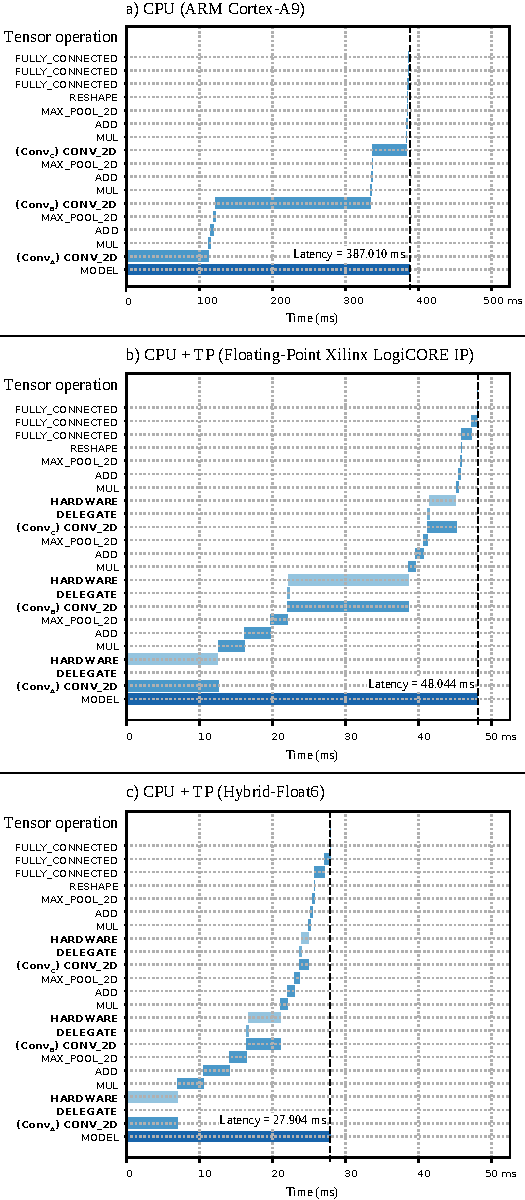
\includegraphics[width=0.5\textwidth]{./chapters/cnn_accelerator/figures/runtime/runtime.pdf}
	\caption{Run-time inference of TensorFlow Lite on the Zynq-7007S SoC. (a) CPU ARM Cortex-A9 at $\unit[666]{MHz}$, (b) cooperative CPU + TP with floating-point Xilinx LogiCORE IP at $\unit[200]{MHz}$, and (c) cooperative CPU + TP with Hybrid-Float6 at $\unit[200]{MHz}$.}
	\label{fig:runtime}
\end{figure}

\subsection{Discussion}
\subsubsection{Training and Quantization}
The training with iterative early stop obtains a model with enhanced accuracy than standard early stop. This method iteratively resets the moving averages of Adam's optimizer, which helps to iteratively search for better local minima. This iterative search is suitable for models with low computational cost.

The TensorFlow Lite 8-bit quantization preserves the overall model accuracy. In some cases, the associated regularization effect can improve the accuracy. However, the error distribution in \gls{cnn} linear regressions gets slightly degraded. In particular, 8-bit quantized output layers incur in discrete-degradation patterns, \fig{fig:2d_error_distribtion}(b) shows this effect on three different models. Vertical and horizontal patterns appear in the error distribution of 8-bit fixed-point quantization. We attribute this effect to the 8-bit resolution in the activation maps. In the case of \gls{hf6} quantization, the activation maps are represented by floating-point preventing this degradation.

The proposed 6-bit \gls{fp} representation (E4M1) improves latency, hardware area, and power dissipation, while preserving model accuracy. For comparison, in our application, this number format produces better results than the 6-bit logarithmic representation (E5M0). This is demonstrated in \Fig{fig:model_evaluation}(d) and \Fig{fig:model_evaluation}(e).

In \cite{lai2017deep}, Lai et al. demonstrated that 4-bit exponent and X-bit mantissa preserves accuracy on SqueezeNet, AlexNet, GoogLeNet, and VGG-16. To contribute on this, I investigated 4-bit exponent and 1-bit mantissa to ALL-CNN-C~\cite{springenberg2014striving}, this produces an accuracy degradation of 1.39\% and 0.11\% with \gls{qat}. While applying 6-bit logarithmic produces a degradation of 11.18\% and 7.22\% with \gls{qat}.

\begin{figure}[t!]
	\centering
	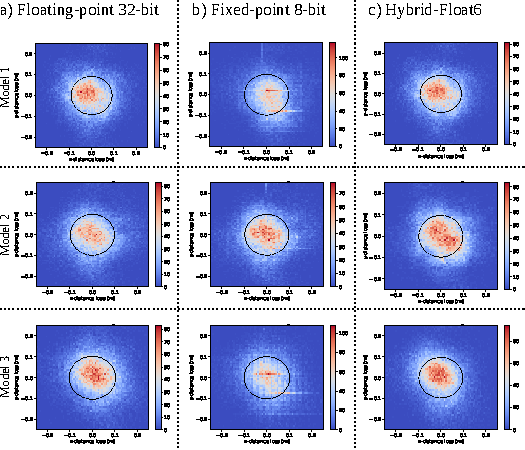
\includegraphics[width=0.5\textwidth]{./chapters/cnn_accelerator/figures/histograms/2D_error_distribtion.pdf}
	\caption{2D error distribution of three CNN-regression models.}
	\label{fig:2d_error_distribtion}
\end{figure}

\subsubsection{Implementation and Performance}
The proposed \gls{hf6} implementation reduces on-chip memory and \gls{dsp} utilization while slightly increasing \glspl{ff} and \glspl{lut} compared to the standard \gls{fp} implementation. See \Tab{tab:resource_utilization} and \Fig{fig:resource_utilization}. This is attributed to the \gls{hf6} logic implementation using \gls{ff} and \gls{lut}, while the \gls{fp} logic implementation uses Xilinx LogiCORE IPs mainly with \glspl{dsp}.

The compute performance of the \gls{cpu} and \gls{tp} on each convolution layer is presented in \Tab{tab:performance} and \fig{fig:acceleration}. 
The peak acceleration and power efficiency of the \gls{tp} with standard \gls{fp} (Xilinx LogiCORE IP) is $13\times$ and \unit[1,558.13]{MFLOPS/s/W}, respectively. While the peak acceleration and power efficiency of the \gls{tp} with \gls{hf6} is $48.3\times$ and \unit[5,743.29]{MFLOPS/s/W}, respectively. The \gls{hf6} hardware demonstrates an improvement of $3.7\times$ in acceleration and power efficiency with respect to the standard \gls{fp} hardware. See \Fig{fig:acceleration}.

The estimated power dissipation on the \gls{soc} is presented in \fig{fig:power}. This shows a very similar breakdown of power dissipation in both implementations. However, the energy efficiency is increased due to the reduced latency in \gls{hf6} hardware. A comparison of related work is presented in \Tab{tab:comparison}.

\begin{figure}[h!]
	\centering
	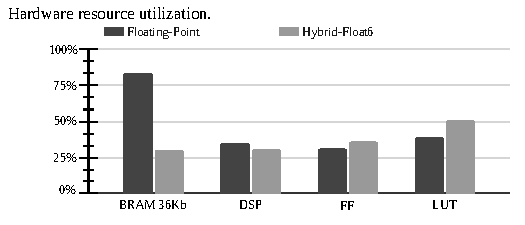
\includegraphics[width=0.5\textwidth]{./chapters/cnn_accelerator/figures/power_breakdown/resource_utilization.pdf}
	\caption{Hardware resource utilization on the Zynq-7007S SoC.}
	\label{fig:resource_utilization}
\end{figure}

\begin{figure}[h!]
	\centering
	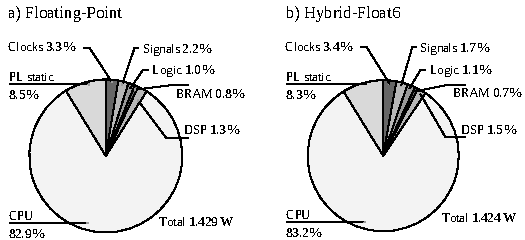
\includegraphics[width=0.5\textwidth]{./chapters/cnn_accelerator/figures/power_breakdown/power_breakdown.pdf}
	\caption{Estimated power dissipation on the Zynq-7007S SoC with PS at $\unit[666]{MHz}$ and PL at $\unit[200]{MHz}$.}
	\label{fig:power}
\end{figure}

The run-time inference of TensorFlow Lite on the \gls{soc} is illustrated in \Fig{fig:runtime}. This shows the convolution layers as the compute-bound operations. The proposed embedded platform is a cooperative system where the convolution operations are delegated to the dedicated hardware accelerator. The ARM \gls{cpu} obtains a latency of $\unit[387]{ms}$ ($\unit[2.58]{FPS}$). The platform with standard \gls{fp} hardware obtains a latency of $\unit[48]{ms}$ ($\unit[20.8]{FPS}$), while the implementation with \gls{hf6} obtains a latency of $\unit[27.9]{ms}$ ($\unit[35.84]{FPS}$). These represent an overall acceleration of $8\times$ and $13.87\times$ over the \gls{cpu}, respectively.

This design facilitates \gls{ml} compatibility/portability as the 6-bit \gls{fp} is wrapped in the standard \gls{fp} representation. The dedicated hardware design extracts the 6-bit format automatically and performs computation.

\subsubsection{SoC Design and Compatibility}
The proposed design is an alternative for high accuracy and low-power floating-point inference. The system runs as a cooperative hardware/software mechanism. This architecture delegates compute-bound tensor operations to a hardware accelerator.

The hybrid 32-bit \gls{fp} and 6-bit \gls{fp} quantization enables high quality of results and backward \gls{ml} compatibility. Backwards \gls{ml} compatibility gives portability from training to inference. This enables to run inference of \gls{hf6} quantized models on standard \gls{fp} hardware and vise versa. The proposed \gls{hf6} architecture allows to compute inference of non-quantized floating-point \gls{ml} models for rapid deployment; however, this will incur in accuracy degradation depending on the resilience of the model, see \Fig{fig:model_evaluation}(c).

\subsubsection{Limitations and Directions for Future Work}
In this research, we foresee three lines of future work:
\begin{itemize}
\item \textbf{To reduce energy consumption.} The proposed architecture consists of a hybrid floating-point quantization using 32-bit activation maps. These can be represented using lower-bit formats; for example, Bfloat16 and 8-bit or lower custom floating-point. This would reduce hardware resource utilization, memory footprint and data transfer, while preserving backward compatibility and accuracy. (Floating-point formats present better \gls{qor} than fixed-pint representations based on the dynamic value range.)

\item \textbf{To increase performance.} This implementation requires matching higher computational throughput with memory bandwidth. This would replace the light-weight pipeline hardware design with a parallelized structure. This will increase hardware area and energy consumption. This can be achieved by using wider memory channels and systolic arrays to increase throughput.

\item \textbf{To use in computer vision applications.} This implementation is designed for sensor analytics workloads. For computer vision applications, the hardware design would require increased on-chip memory capacity for larger bias and filter vectors (using equations from Section \ref{sec:memory_utilization}), and higher computational throughput in a larger/costlier \gls{fpga} \gls{soc}.
\end{itemize}

\begin{table*}[!t]\centering
	\caption{Comparison of hardware implementation with related work.}\label{tab:comparison}
	\scriptsize
	\begin{tabular}{lrrrrrr}\toprule
		Platform &Chunsheng Mei et al. \cite{mei2017200mhz} &Chen Wu et al. \cite{wu2021low} &BFP \cite{lian2019high} &Paolo Meloni et al. \cite{meloni2019cnn} &This work \\\midrule
		Device &XC7VX690T &XC7K325T &XC7VX690T &XC7Z007S &XC7Z007S \\
		Year &2017 &2019 &2019 &2019 &2022 \\
		Dev. kit cost &\$7,494 &\$1,299 &\$7,494 &\$89 &\$89 \\
		Format (activation/weight) &FP 16-bit &FP 8-bit / 8-bit &FP 16-bit / 8-bit &INT 16-bit &FP 32-bit / 6-bit \\
		Frequency (MHz) &200 &200 &200 &80 &200 \\
		Peak power efficiency (GFLOP/s/W) &18.72 &115.40 &82.88 &2.98 &5.74 \\
		Peak throughput (GFLOP/s) & 202.42 & 1086.8 & 760.83 &  10.62& 0.482\\
		Wall plug power (W) &10.81 &9.42 &9.18 &2.5 &2.3 \\
		BRAM 36Kb utilization &196.5 &234.5 &913 &44 &15 \\
		DSP utilization &1728 &768 &1027 &54 &20 \\
		\bottomrule
	\end{tabular}
\end{table*}
\section{Conclusions}
\label{sec:conclusions}
In this paper, we present the Hybrid-Float6 quantization for floating-point CNN hardware acceleration. Feature maps and weights are represented by 32-bit and 6-bit floating-point, respectively. The 6-bit floating-point format is composed of 1-bit sign, 4-bit exponent, and 1-bit mantissa. The 1-bit mantissa enables low-power multiply-accumulate implementations by reducing the mantissa multiplication to a multiplexer-adder operation. We exploit the intrinsic error tolerance of neural networks to further reduce the hardware design with approximation. This approach improves latency, hardware area, and energy consumption. To preserve accuracy, we introduce a quantization aware training method that, in some cases, improves accuracy. We present a lightweight tensor processor implementing a pipelined vector dot-product. For ML compatibility/portability, the 6-bit FP is wrapped in the standard floating-point format, which is automatically extracted by the proposed hardware. The hardware/software architecture is compatible with TensorFlow Lite. We evaluate the applicability of our approach with a CNN-regression model for anomaly localization in a structural health monitoring application based on acoustic emissions. The embedded hardware/software framework is demonstrated on XC7Z007S as the smallest Zynq-7000 SoC. The proposed hardware achieves a peak power efficiency and acceleration on convolution layers of $5.7$ GFLOPS/s/W and $48.3\times$, respectively.
\section{SbS algorithm}
\label{chap:appendix}

The SbS network inference is described in \Algo{alg:inference}, while spike production and layer update are described in \Algo{alg:spike} and \Algo{alg:update}, respectably.

\begin{algorithm}[t]
	\caption{SbS network inference.} \label{alg:inference}
	
	\begin{algorithmic}
		\SetAlgoLined
		\renewcommand{\algorithmicrequire}{\textbf{input:}}
		\renewcommand{\algorithmicensure}{\textbf{output:}}
		\REQUIRE Layers of the network as $H^l$, where\\
		$l$ is the layer index.
		\REQUIRE $N_{L}$ as the number of layers.
		\REQUIRE $N^l_{X}, N^l_{Y}$ as the size of layers.
		\REQUIRE $N_{Spk}$ as the number of spikes for inference (iterations).
		\ENSURE $H^l$.
		\FOR {$t = 0$ \textbf{to} $N_{Spk}-1$}
		\STATE \textit{Initialization of $H^l(i_X,i_Y,:)$} :
		
		\IF {$t == 0$}
		\FOR {$l = 0$ \textbf{to} $N_{L}-1$}
		\FOR {$i_X = 0, i_Y = 0$ \textbf{to} $N^l_{X}-1, N^l_{Y}-1$}
		\FOR {$i_{H} = 0$ \textbf{to} $N^l_H-1$}
		\STATE $H^l(i_X,i_Y,i_{H}) = 1/N^l_H$
		\ENDFOR
		\ENDFOR
		\ENDFOR
		\ENDIF
		
		\textit{Production of spikes} :
		
		\FOR {$l = 0$ \textbf{to} $N_{L}-1$}
		\IF {$l == 0$}
		\STATE Draw spikes from input \tcp{(Algorithm~\ref{alg:spike})}
		\ELSE
		\STATE Draw spikes from $H^l$ \tcp{(Algorithm~\ref{alg:spike})}
		\ENDIF
		
		\ENDFOR
		
		\textit{Update layers} :
		\FOR {$l = 0$ \textbf{to} $N_L - 1$}
		\STATE Update $H^l$ \tcp{(Algorithm~\ref{alg:update})}
		\ENDFOR
		
		\ENDFOR
	\end{algorithmic} 
\end{algorithm}


\begin{algorithm}[t]
	\caption{Spike production.} \label{alg:spike}
	
	\begin{algorithmic}[1]
		\SetAlgoLined
		\renewcommand{\algorithmicrequire}{\textbf{input:}}
		\renewcommand{\algorithmicensure}{\textbf{output:}}
		\REQUIRE Layer as $H_t\in\mathbb{R}^{N_X \times N_Y \times N_H}$, where\\
		$N_X$ is the layer width,\\
		$N_Y$ is the layer height\\
		$N_H$ is the length of $\vec{h}$ (IP vector).
		\ENSURE Output spikes as $S_t^{out} \in\mathbb{N}^{N_X \times N_Y}$
		
		\FOR {$i_X = 0$, $i_Y = 0$ \textbf{to} $N_X-1$, $N_Y-1$}
		
		
		\STATE \textit{Generate spike} :
		
		\STATE $th = MT19937PseudoRandom()/(2^{32}-1)$
		\STATE $acu = 0$
		\FOR {$i_{H} = 0$ \textbf{to} $N_H-1$}
		\STATE $acu = acu + H_t(i_X,i_Y,i_{H})$
		\IF {$th \leq acu$ \textbf{or} $i_{H} == N_{H}-1$}
		\STATE $S_t^{out}(i_X,i_Y) = i_{H}$
		\ENDIF
		\ENDFOR
		\ENDFOR
	\end{algorithmic} 
\end{algorithm}





\begin{algorithm}[t]
	\caption{SbS layer update.} \label{alg:update}
	
	\begin{algorithmic}[1]
		\SetAlgoLined
		\renewcommand{\algorithmicrequire}{\textbf{input:}}
		\renewcommand{\algorithmicensure}{\textbf{output:}}
		\REQUIRE Layer as $H\in\mathbb{R}^{N_X \times N_Y \times N_H}$, where\\
		$N_X$ is the layer width,\\
		$N_Y$ is the layer height\\
		$N_H$ is the length of $\vec{h}$ (IP vector).
		\REQUIRE Synaptic matrix as $W\in\mathbb{R}^{K_X \times K_Y \times M_H\times N_H}$, where\\
		$K_X \times K_Y$ is the size of the convolution/pooling kernel, \\
		$M_H$ is the length of $\vec{h}$ from previous layer,\\
		$N_H$ is the length of $\vec{h}$ from this layer.  
		\REQUIRE Input spike matrix from previous layer as $S_t^{in} \in\mathbb{N}^{N_{Xin} \times N_{Yin}}$, where\\
		$N_{Xin}$ is the width of the previous layer,\\
		$N_{Yin}$ is the height of the previous layer.
		\REQUIRE Strides of X and Y as $stride_{X}$ and $stride_{Y}$, respectively.
		
		\REQUIRE Epsilon as $\epsilon\in\mathbb{R}$.
		\ENSURE Updated layer as $H^{new}\in\mathbb{R}^{N_X \times N_Y \times N_H}$.
		\\
		\textit{Update layer} :
		\STATE $z_{X} = 0$ \tcp{X and Y index for $S_t^{in}$}
		\STATE $z_{Y} = 0$
		\FOR {$i_Y = 0$ \textbf{to} $N_Y - 1$}
		\FOR {$i_X = 0$ \textbf{to} $N_X-1$}
		\STATE $\vec{h} = H(i_X, i_Y,:)$\\
		
		\textit{Update IP} :
		\FOR {$j_X = 0, j_Y = 0$ \textbf{to} $K_X - 1,K_Y - 1$}
		
		\STATE $s_t = S_t^{in}(z_{X}+j_X,z_{Y}+j_Y)$
		\STATE $\vec{w} = W(j_X,j_Y,s_t,:)$
		\STATE $\vec{p} = 0$
		
		\textit{Dot-product} :
		\STATE $r = 0$
		\FOR {$j_H = 0$ \textbf{to} $N_H-1$}
		\STATE $\vec{p}(j_H) = \vec{h}_(j_H)\vec{w}(j_H)$
		\STATE $r = r + \vec{p}(j_H)$
		\ENDFOR
		
		
		\IF {$r \ne 0$}
		\STATE \textit{Update IP vector} :
		\FOR {$i_H =$ \textbf{to} $N_H-1$}
		\STATE
		$  h^{new}(i_H) = \frac{1}{1+\epsilon} \left(h(i_H) + \epsilon \frac{\vec{p}(i_H) }{r} \right) $
		\ENDFOR
		
		\textit{Set the new $H$ vector for the layer} :
		\STATE $H^{new}(i_X,i_Y,:) = \vec{h}^{new}$
		\ENDIF
		\ENDFOR
		\STATE $z_{X} = z_{X} + stride_{X}$
		\ENDFOR
		\STATE $z_{Y} = z_{Y} + stride_{Y}$
		\ENDFOR
		
	\end{algorithmic} 
\end{algorithm}




\bibliographystyle{IEEEtran}
\bibliography{../content/bibliography.bib}

\begin{IEEEbiography}[{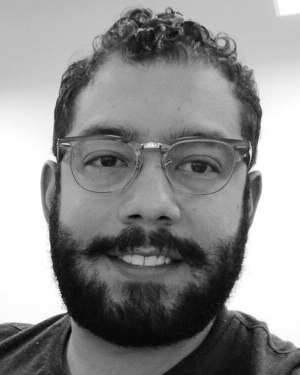
\includegraphics[width=1in,height=1.25in,clip,keepaspectratio]{../biography/yarib_300_375.jpg}}]{Yarib Nevarez} received the B.E. (Hons) degree in electronics from the Durango Institute of Technology, Durango, Mexico, in 2009, and the M.Sc. degree in Embedded Systems Design from the University of Applied Sciences Bremerhaven, Bremen, Germany, in 2017. He is currently pursuing a PhD degree with the Institute of Electrodynamics and Microelectronics, University of Bremen, Germany. His research interest is focused mainly on System-on-Chip architectures and hardware implementation for deep learning accelerators in Embedded Systems.
\\
During his professional experience, he served as a Senior Embedded Software Engineer at Texas Instruments, IBM, Continental Automotive, TOSHIBA, and Carbon Robotics. He has designed and developed software architectures for graphic calculators, automotive systems, robotic drivers, and more.
	
\end{IEEEbiography}

\begin{IEEEbiography}[{
\includegraphics[width=1in,height=1.25in,clip,keepaspectratio]{../biography/Beering_bw_klein.jpeg}}]{Andreas Beering} received his B.Sc. and M.Sc. degree in Electrical and Information Engineering  from the University of Bremen, Germany, in 2015 and 2017, respectively. He is currently working towards a Ph.D. degree at the Institute of Electrodynamics and Microelectronics at the University of Bremen, Germany. His research interests focus mainly on signal processing and classification of vibration signals. In addition to the analysis of passive acoustic emission for monitoring gearboxes and processes, the second focus lies on active ultrasonic investigations.
In this context, ultrasonic waveforms for monitoring overmoulding processes are being investigated.
\end{IEEEbiography}

\begin{IEEEbiography}[{
\includegraphics[width=1in,height=1.25in,clip,keepaspectratio]{../biography/person.png}}]{Amir Najafi}
\end{IEEEbiography}

\begin{IEEEbiography}[{
\includegraphics[width=1in,height=1.25in,clip,keepaspectratio]{../biography/person.png}}]{Ardalan Najafi}
\end{IEEEbiography}

\begin{IEEEbiography}[{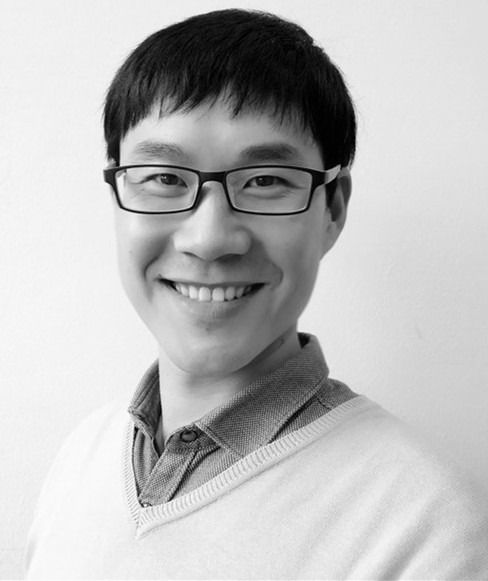
\includegraphics[width=1in,height=1.25in,clip,keepaspectratio]{../biography/wyu.jpg}}]{Wanli Yu}
	
	received the B. S. degree in information engineering and the M. S. degree in signal and information processing from the China University of Mining and Technology, Xuzhou, China, in 2009 and 2012, respectively and the PhD degree from the University of Bremen, Germany, in 2018.
	
	He is currently a Post-Doctoral Researcher with the Institute of Electrodynamics and Microelectronics, University of Bremen. His research interests include sensor networks, Internet of Things, network performance optimization, energy aware task allocation and scheduling, mobile edge/fog computing, convex optimization, machine learningand nature-inspired population-based optimization.
\end{IEEEbiography}

\begin{IEEEbiography}[{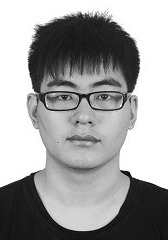
\includegraphics[width=1in,height=1.25in,clip,keepaspectratio]{../biography/YizhiChen.jpg}}]{Yizhi Chen} received the B.E. degree in Electronic and Information Engineering from Wuhan University, China, in 2017 and he received the M.S. degree in Communication and Information Technology from the University of Bremen, Germany, in 2021. Currently, he is working as a Ph.D. student at the Division of Electronics and Embedded Systems, Department of Electrical Engineering, School of Electrical Engineering and Computer Science, KTH Royal Institute of Technology, Sweden. His research interests include hardware accelerator for ML, fault-tolerant hardware for neural networks, Network-on-Chip, and approximate computing.
\end{IEEEbiography}

\begin{IEEEbiography}[{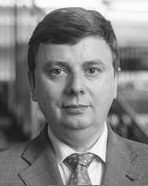
\includegraphics[width=1in,height=1.25in,clip,keepaspectratio]{../biography/krieger.jpg}}]{Karl-Ludwig Krieger} received his Ph.D. degree in Electrical Engineering in 1999 from the University of Bremen, Germany. Dr. Krieger worked from 1998-2009 as a manager in the field of function and algorithm development for powertrain systems at Daimler AG in Stuttgart. Since 2009 he has been a full professor for the chair of Electronic Vehicle and Mobility Systems at the University of Bremen, Germany. The research focus of his chair is primarily on the analysis of vibration and ultrasound signals in different application fields, for example, passenger cars, heavy-duty trucks, mobile working machines or industrial machines. Further research priorities of the chair are near-infrared spectral sensors and capacitive sensor systems for different fields of application. These research topics are worked on in close cooperation with leading industrial partners and are mainly financed from third-party funds.
\end{IEEEbiography}

\begin{IEEEbiography}[{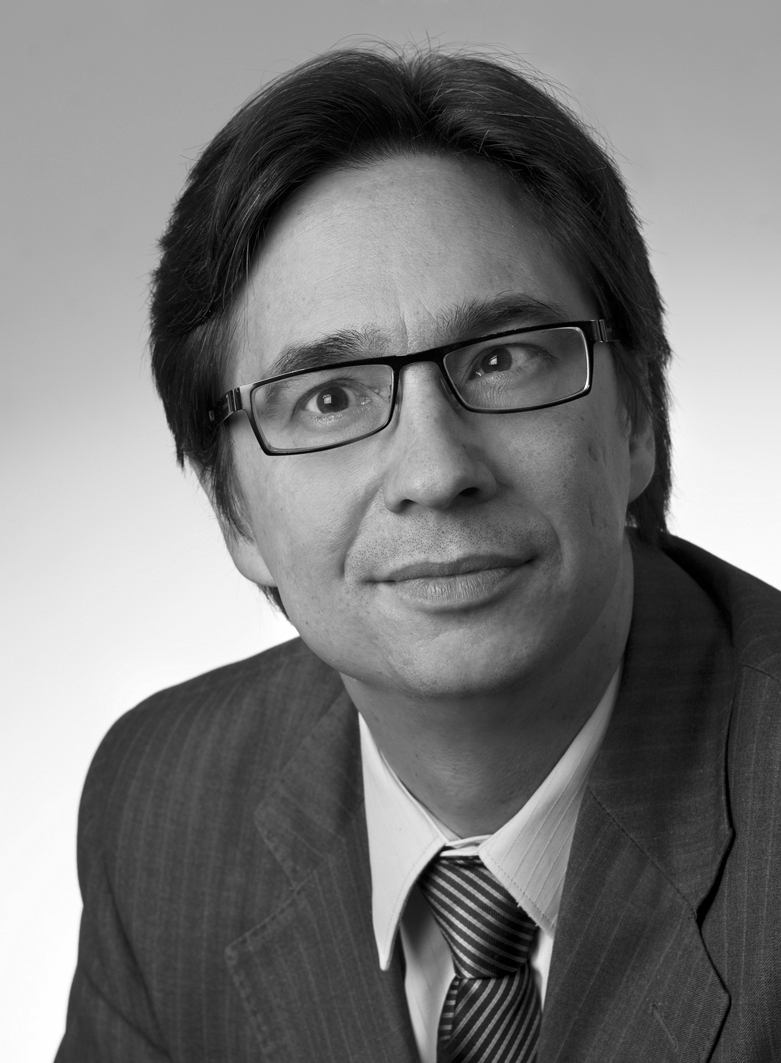
\includegraphics[width=1in,height=1.25in,clip,keepaspectratio]{../biography/Alberto_Garcia-Ortiz.jpg}}]{Alberto Garcia-Ortiz}
    obtained the diploma degree in
    Telecommunication Systems from the Polytechnic University of
    Valencia (Spain) in 1998. After working for two years at Newlogic
    in Austria, he started the Ph.D. at the Institute of
    Microelectronic Systems, Darmstadt University of Technology,
    Germany. In 2003, he received from the Department of Electrical
    Engineering and Information Technology of the university the
    Ph.D. degree with "summa cum laude." From 2003 to 2005, he worked
    as a Senior Hardware Design Engineer at IBM Deutschland
    Development and Research in B{\"o}blingen.  After that he joined the
    start-up AnaFocus (Spain), where he was responsible for the design
    and integration of AnaFocus" next generation Vision
    Systems-on-Chip. He is currently full professor for the chair of
    integrated digital systems at the university of Bremen.
    Dr. Garcia-Ortiz received the "Outstanding dissertation award" in
    2004 from the European Design and Automation Association. In 2005,
    he received from IBM an innovation award for contributions to
    leakage estimation. Two patents are issued with that work. He
    serves as editor of JOLPE and is reviewer of several conferences,
    journals, and European projects. \\
    His interests include low-power
    design and estimation, communication- centric design, SoC
    integration, and variations-aware design. 
\end{IEEEbiography}


\EOD

\end{document}
